
% LTeX: language=fr
%%%%%%%%%%%%%%%%%%%%%%%%%%%%%%%%%%%%%%%%%%%%%%%%%%%%%%%%%%%%%%%%%%%
%%%                       CHAPITRE 4                            
%%%%%%%%%%%%%%%%%%%%%%%%%%%%%%%%%%%%%%%%%%%%%%%%%%%%%%%%%%%%%%%%%%%

\lhead[\fancyplain{}{\leftmark}]%Pour les pages paires \bfseries
      {\fancyplain{}{}} %Pour les pages impaires
\chead[\fancyplain{}{}]%
      {\fancyplain{}{}}
\rhead[\fancyplain{}{}]%Pour les pages paires 
      {\fancyplain{}{\rightmark}}%Pour les pages impaires \bfseries
\lfoot[\fancyplain{}{}]%
      {\fancyplain{}{}}
\cfoot[\fancyplain{}{\thepage}]%\bfseries
      {\fancyplain{}{\thepage}} %\bfseries
\rfoot[\fancyplain{}{}]%
     {\fancyplain{}{\scriptsize}}

%/!\/!\/!\/!\/!\/!\/!\/!\/!\/!\/!\/!\/!\/!\/!\/!\/!\/!\/!\/!\/!\/!\/!\/!\ SECTION
    %///////////////////////////////////////////// sous-section
    		%************* sous-sous-section
    					 %--------- paragraphe    		


%%%%%%%%%%%%%%%%%
%\begin{table}[!htbp]
%\centering
%%\rowcolors[]{2}{black!8}{}{
%\renewcommand{\arraystretch}{2}
%\begin{tabular}{c c c}
%\rowcolor{blue!10}
%Paramètre & Symbole & Valeur numérique \\
%\hline
%\hline
%Flambement OB seul & $x_{0,eq}$ &  0.55mm \\ 
%\hline
%Rigidité VH  & $K_{T40}$ & 0.48Nmm/rad \\ 
%\hline
%Flambement OBVH & $x_{0}$ &  0.49mm \\ 
%\hline
%Bras de levier de VH & $zlat_{eq}$ & 1.9mm \\
%\hline
%\end{tabular}
%\label{tab:recalage_OBVH}
%\end{table}
%%%%%%%%%%%%%%%%%
    					 
%%%%%%%%%%%%%%%%%%%%%%%%%%%%%%%%%%%%%%%%%%%%%%%%%%%%%%%%%%%%%%%%%%%%%%%%%%
%%%%%                      Start part here                          %%%%%%
%%%%%%%%%%%%%%%%%%%%%%%%%%%%%%%%%%%%%%%%%%%%%%%%%%%%%%%%%%%%%%%%%%%%%%%%%%

\chapter{Valves hydrauliques à base de tubes flexibles flambés}
\label{ch:4_Valves hydrauliques a base de tubes flexibles flambes}

\minitoc
\newpage

%/!\/!\/!\/!\/!\/!\/!\/!\/!\/!\/!\/!\/!\/!\/!\/!\/!\/!\/!\/!\/!\/!\/!\/!\ 
\section{Stratégie d'approches}
\label{sec:4.1 - Strategie d approches}
%/!\/!\/!\/!\/!\/!\/!\/!\/!\/!\/!\/!\/!\/!\/!\/!\/!\/!\/!\/!\/!\/!\/!\/!\
	%/////////////////////////////////////////////
	\subsection{Rappel du cahier des charges}
	\label{subsec:4.1.1 - Rappel du cahier des charges}
    %/////////////////////////////////////////////
\lettrine[lines=1]{L~}{}e chapitre \ref{ch:2_Modelisation et simulation du systeme} a mis en évidence le besoin du cyclage dans le fonctionnement de l'OB. Ce-dernier nécessite un actionnement bi-directionnel par le biais de deux PH. Cela nécessite alors un dispositif de gestion du fluide sortant du bouchon d'oreille, pour alimenter les deux pistons de façon alternative. Après étude du besoin, nous avons conclu que ce rôle pouvait être assuré par deux VH. Naturellement, la position ouverte ou fermée des VH doit dépendre de façon antisymétrique de la position de la masse afin d’assurer le bon cyclage de l'OB.

Nous avons alors établi dans la section \ref{sec:2.2_Cyclage du mouvement de la masse dynamique du bistable : valves hydrauliques} le cahier des charges pour les VH. Entre autres, le critère hydraulique impose que les PdC dans la VH fermée soient suffisamment élevées afin de couper l'alimentation en fluide du piston fermé. Puis, le critère énergétique exige que l'énergie mécanique requise pour la commutation des VH soit négligeable par rapport à l'énergie produite, afin de maximiser le rendement de conversion global du récupérateur d'énergie.

La solution technologique retenue pour les VH est un tube flexible amené en flexion au-delà de sa limite de flambement. La réduction de diamètre hydraulique ainsi engendrée au niveau de la section flambée doit alors générer suffisamment de pertes de charges pour assurer l'écoulement vers la branche ouverte. Cela se traduit par un rapport $r_{Cf}$ (éq. \ref{eq:r_Cf}) devant être supérieur à 10 d'après les simulations préliminaires présentées dans la sous-section \ref{subsec:2.5.3:Simulation et resultats}. Deux stratégies vont alors être exposées pour le développement de VH en accord avec ce CdC. La première est expérimentale et sera discutée dans ce chapitre. La seconde est plutôt théorie et fera l'objet du chapitre suivant. Enfin, une corrélation sera réalisée par la suite entre les deux approches et les résultats seront discutés.
	%/////////////////////////////////////////////
	\subsection{Stratégies}
	\label{subsec:4.1.2 - Strategies}
    %/////////////////////////////////////////////
L'objectif de la thèse est de présenter une nouvelle approche pour exploiter l'énergie de déformation mécanique du conduit auditif. La conversion d'énergie au travers de l'OB implémentant un GPA a déjà été étudiée et montrée dans la littérature. L'élément dont le fonctionnement reste à valider est le comportement des VH à base de tubes flambés. Une telle étude n'a pas encore été proposée par la communauté de chercheurs concernés. Par conséquent, il n'existe, à notre connaissance, aucun modèle théorique exploitable. En revanche, on sait qualitativement que le phénomène d'étranglement hydraulique est notable dans un écoulement rencontrant une section flambée de tube en flexion (fig. \ref{fig:tuyau_arrosage}).

Pour répondre aux besoins du système, deux approches sont envisageables. Une première approche pourrait être théorique, en vue d'estimer les comportements statiques et hydrauliques des tubes flexibles en flambement. Cela nécessiterait cependant une validation expérimentale.\\
Une approche alternative pourrait être l'étude empirique des comportements statiques et hydrauliques des VH à base de tubes flambés. Un modèle prédictif pourrait alors être établi à partir des données expérimentales. Cette approche permettrait de valider la faisabilité d'une telle solution, car elle reflète directement le comportement réel des VH.

Dans la suite de ce chapitre, sera considérée l'approche empirique pour la caractérisation des VH. 
%/!\/!\/!\/!\/!\/!\/!\/!\/!\/!\/!\/!\/!\/!\/!\/!\/!\/!\/!\/!\/!\/!\/!\/!\  
\section{Caractérisation expérimentale de la raideur d'une VH}
\label{sec:4.2_Caracterisation experimentale de K_VH}
%/!\/!\/!\/!\/!\/!\/!\/!\/!\/!\/!\/!\/!\/!\/!\/!\/!\/!\/!\/!\/!\/!\/!\/!\ 
Nous avons établi trois critères de validité, pour le fonctionnement des VH, qu'on peut résumer comme suit :
\begin{itemize}[label=$\blacksquare$]
	\item \emph{Critère statique} : L'énergie nécessaire pour plier une VH doit être négligeable devant l'énergie disponible dans l'OB.
	\item \emph{Critère hydraulique} : Les pertes de charges induites par la VH fermée doivent favoriser l'écoulement dans la branche opposée.
	\item \emph{Critère de cyclage} : L'intégration des VH doit se faire de façon à ce que leur comportement soit antisymétrique par rapport à la position $x_m=0$ de la masse.
\end{itemize} 
Tout d'abord, il est nécessaire d'établir les paramètres matériau et géométriques du tube flexible remplissant le critère énergétique du fonctionnement d'une VH. Ensuite, il faudra caractériser le comportement hydraulique à travers la section flambée du tube validant le critère précédent. Le critère de cyclage sera discuté, mais l'intégration complète expérimentale de VH en fonctionnement rentrera dans les perspectives des travaux de thèse.
    %///////////////////////////////////////////// 		
	\subsection{Raideur de VH admissible pour l'OB}
	\label{subsec:4.2.1_Raideur de VH admissible pour l'OB}
    %/////////////////////////////////////////////	   
Afin d'estimer l'ordre de grandeur de la raideur acceptable pour une VH, nous nous basons sur la limite de bistabilité du prototype monobloc présenté dans le chapitre précédent. Comme évoqué dans la section \ref{sec:3.3.1_Limite structurelle et précontrainte de flambement}, l'OB seul admet une hauteur de flambement maximale $x_{0,max} = 0.63mm$ assurant une meilleure efficacité de conversion d'énergie. L'équilibre statique de L'OB initialement flambé au niveau $x_{0,max}$, avec la prise en compte de l'influence mécanique de la VH, s'exprime à travers l'équation \ref{eq:equilibre statique a x0_max}.
\begin{equation}
 \frac{K\ {x_{0,max}}^2}{L^2}\biggl(\frac{{x_{0,vh}}^2}{{x_{0,max}}^2} -1\biggr)x_{0,vh} - \biggl( \frac{K_{VH}}{a} \biggr) \arctan \biggl(\frac{x_{0,vh}}{a} \biggr) = 0
	\label{eq:equilibre statique a x0_max}
\end{equation}
La bistabilité de l'ensemble OB + VH (OBVH) est assurée si l'équation \ref{eq:equilibre statique a x0_max} admet deux positions stables $\pm x_{0,vh}$ qui sont fonction de $K_{VH}$, supposé ici indépendant de $x_m$.
%%%%%%%%%%%%%%%%%%%%%%%%%%%%%%%%%%%%	
\begin{figure}[!htb]
	\begin{center}
		\captionsetup{justification=centering}
		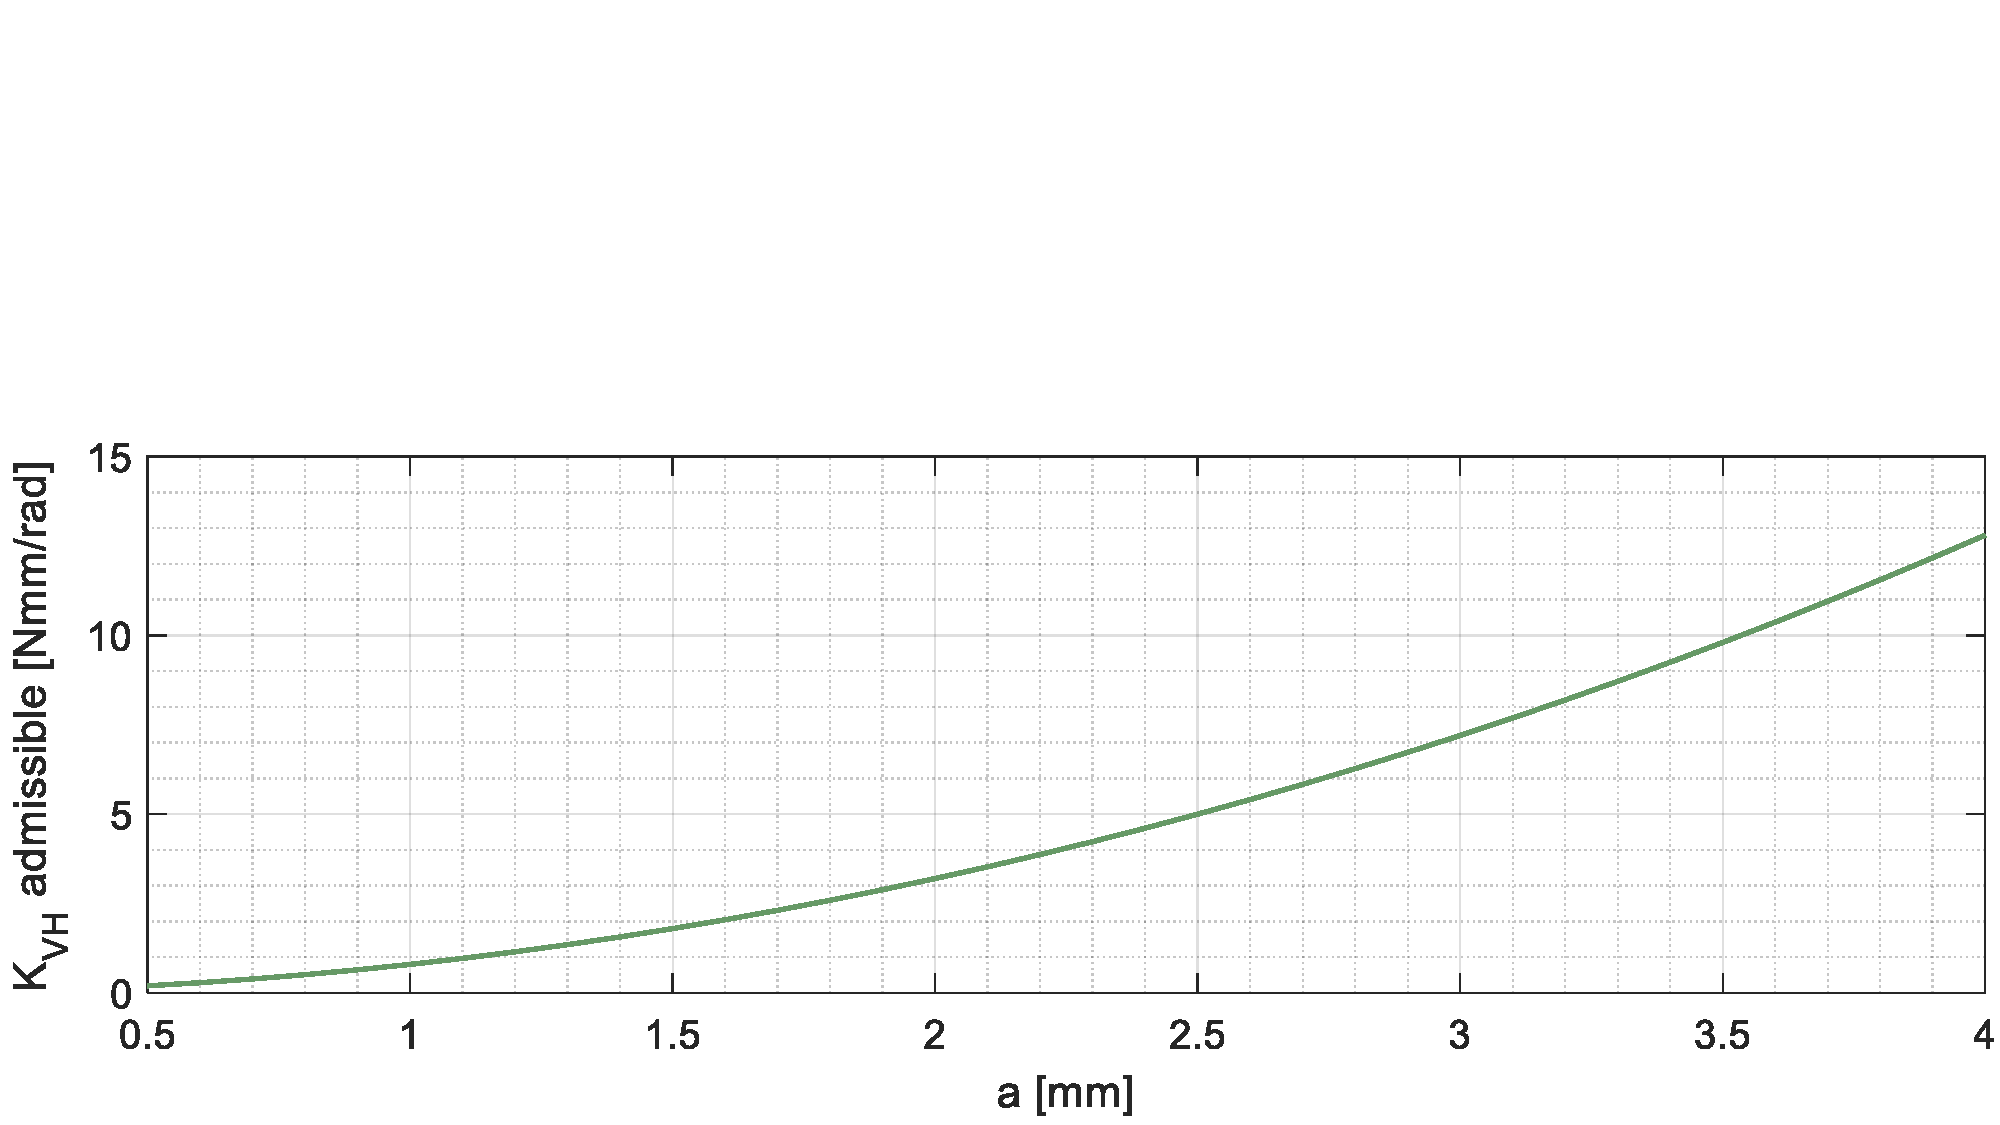
\includegraphics[trim={0cm 0cm 0cm 7cm},clip,width=0.8\textwidth]{../Chap4/Figure/(K_VH)_max(a)_bistabilite.pdf}
		\caption{Raideur $K_{VH}$ admissible afin d'assurer la bistabilité de l'OB dimensionné pour $x_0=x_{0,max}$.}
		\label{fig:(K_VH)_max(a)_et_Deltatheta_pour_bistabilite}
	\end{center}
\end{figure}    
%%%%%%%%%%%%%%%%%%%%%%%%%%%%%%%%%%%%

On ne connaît pas le bras de levier $a$ pour le pliage de la VH mais on sait néanmoins que sa valeur se situe dans l'ordre de grandeur millimétrique, en cohérence avec $x_{0,max} = 0.63mm$. La figure \ref{fig:(K_VH)_max(a)_et_Deltatheta_pour_bistabilite} montre alors l'évolution de la raideur maximale admissible pour l'OB présenté dans le chapitre précédent, en tenant compte des défauts de fabrication. Au-delà de la valeur admissible, pour $a$ donné, l'oscillateur devient monostable en $x=0$. La valeur de $K_{VH}$ devra donc être très faible devant sa valeur admissible pour un bras de levier donné. Par ailleurs, pour maximiser la raideur admissible pour une VH, il faut augmenter $a$. En revanche, en nous appuyant sur l'équation \ref{eq:theta=f(x_m)}, on sait que pour maximiser $\Delta\theta$ il faudra diminuer $a$. Un compromis sur la valeur de $a$ sera donc nécessaire pour un fonctionnement optimal.
    %///////////////////////////////////////////// 		
	\subsection{Choix du matériau}
	\label{subsec:4.2.2_Choix du matériau}
    %/////////////////////////////////////////////	       
Le choix du matériau est la première chose à considérer. Les matériaux souples sont les plus propices pour limiter la rigidité en rotation du tube. Les familles des polymères et silicones sont en effet des choix de matériaux à considérer pour notre application. Il faut noter que le choix des matériaux impose certains diamètres et épaisseurs disponibles auprès des fournisseurs.

La cinématique réelle du pliage du tube a été illustrée sur la figure \ref{fig:detail_flambement_MDOB}. Il a été intéressant de procéder à un essai qualitatif de pliage de tubes,  suivant cette configuration, pour différents matériaux et différentes géométries. Les photos de la figure \ref{fig:materiaux_tubes_plies} montrent les résultats de ces essais et le tableau \ref{tab:parametres_tubes_tests_qualitatifs} donne les valeurs de diamètre intérieur $D_t$, épaisseur $th_t$ et l'ordre de grandeur du module d'Young $E_t$ pour chaque tube. Nous avons testé 3 matériaux : le kapton, le polyéthylène et le silicone. Les échantillons de tubes ont été fixés parallèlement à l'axe $\vec{x}$, dans deux gaines rigides à chaque extrémité. La partie droite a été encastrée dans un support fixe et la partie gauche est soumise, au contact d'une masse mobile, à un déplacement suivant $\vec{x}$. Les images montrent les tubes en flexion après le déplacement de la masse mobile suivant $\vec{x}$. $\theta$ est défini comme l'angle formé par l'intersection des axes des sections $S_1$ et $S_2$ des gaines rigides.
%%%%%%%%%%%%%%%%%%%%%%%%%%%%%%%%%%%%%%%%%%%%%
\begin{figure}[ht!]
	\begin{center}
		\captionsetup{justification=centering}
		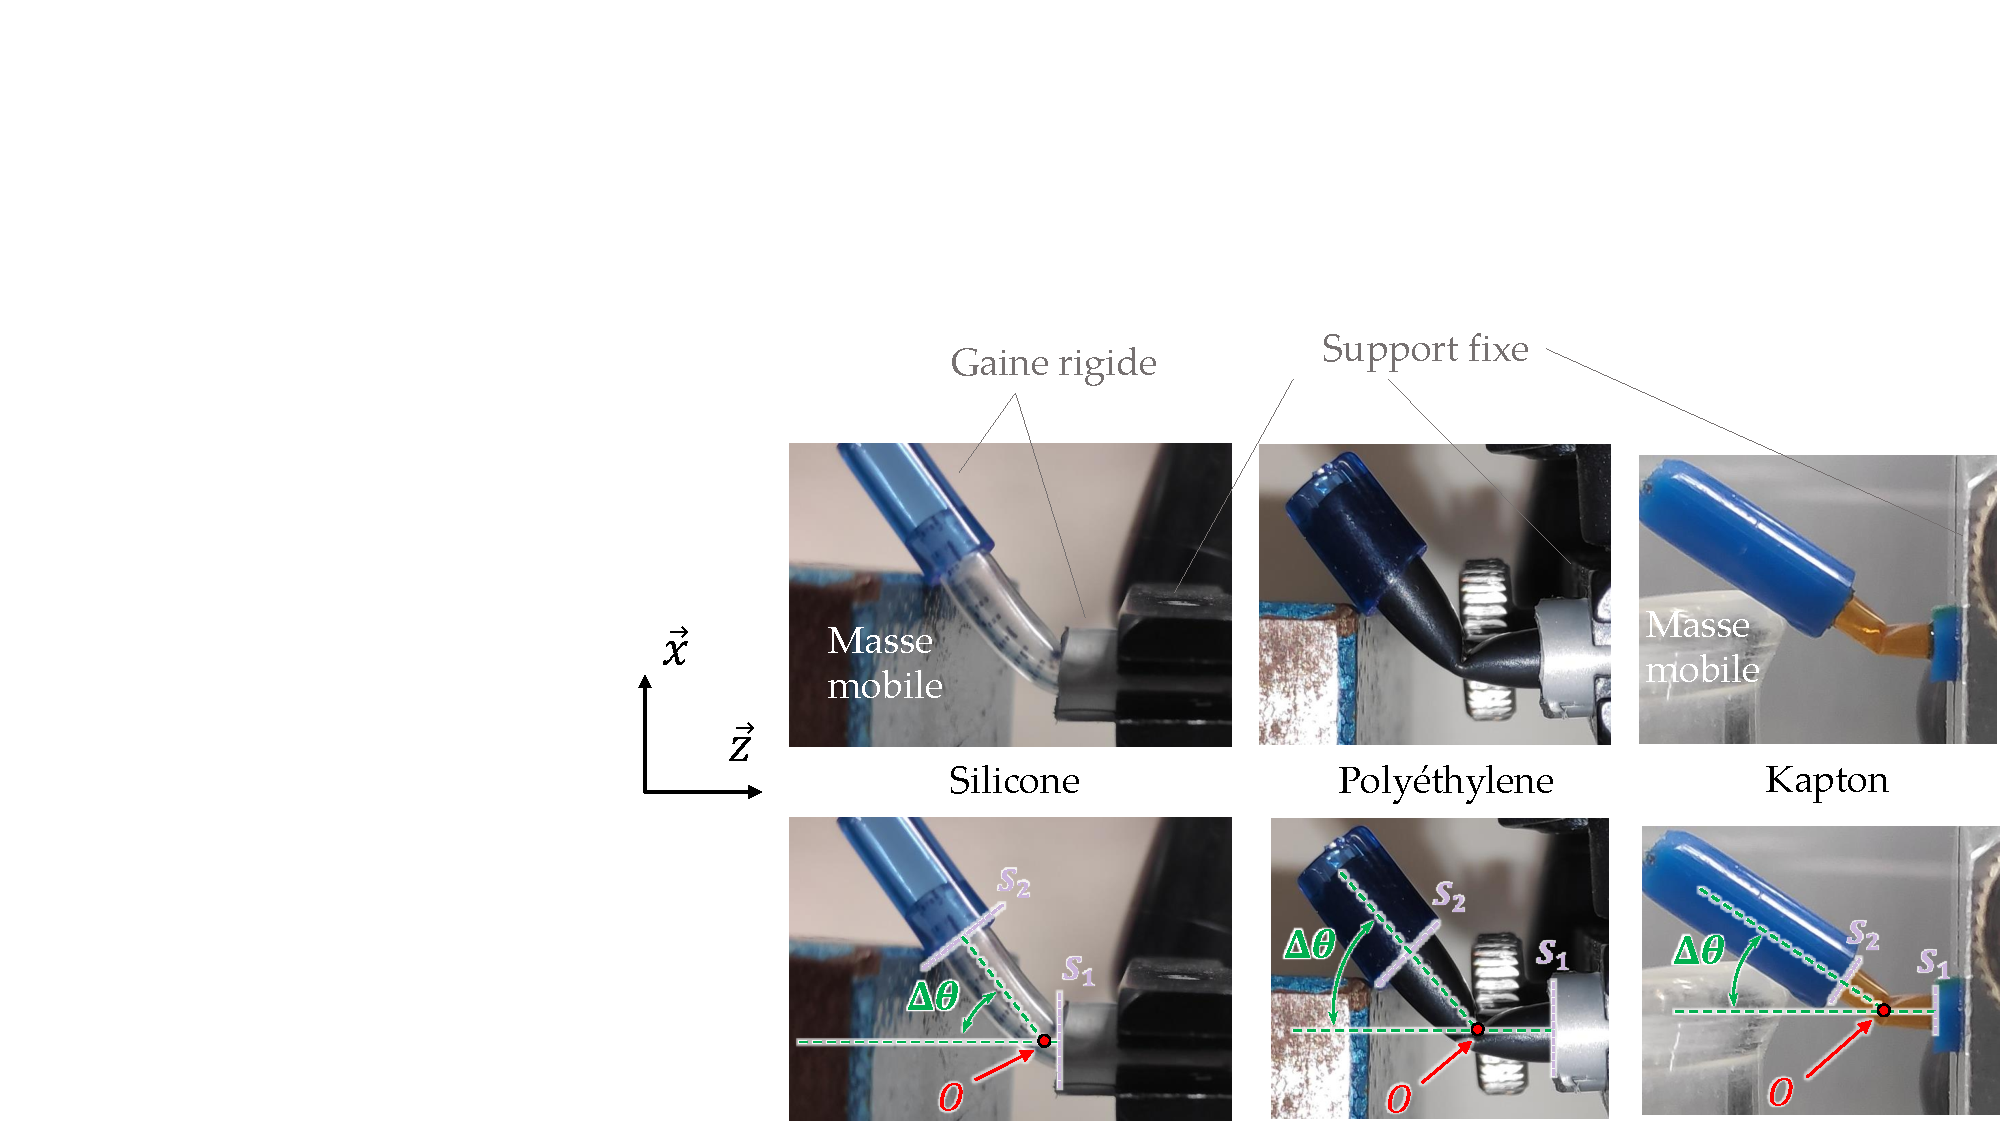
\includegraphics[trim={10.5cm 0cm 0cm 5.5cm},clip,width=0.8\textwidth]{../Chap4/Figure/materiaux_tubes_plies.pdf}
		\caption{Estimation qualitative de l'étranglement pour 3 tubes de matériaux et géométries différents}
		\label{fig:materiaux_tubes_plies}
	\end{center}
\end{figure}
%%%%%%%%%%%%%%%%%%%%%%%%%%%%%%%%%%%%%%%%%%%%%
%%%%%%%%%%%%%%%%%%%%%%%%%%%%%%%%%%%%%%%%%%%%%
\begin{table}[!htbp]
	\centering
	\captionsetup{justification=centering}
	\rowcolors[]{2}{black!8}{}{
	\begin{tabular}{c|c|c|c}
		\rowcolor{blue!10}
		\toprule
		\textbf{\emph{Paramètre}~~[Unité]} & \textbf{Silicone} & \textbf{Polyéthylène } & \textbf{Kapton} \\
		\midrule
		$D_t~~$	[mm]                       & 3                 & 3.5                    & 2               \\
		$th_t~~$[mm]                       & 1                 & 0.5                    & 0.025           \\
		$E_t~~$[GPa]                       & 0.03              & 0.2-0.7                & 2-5             \\
		\bottomrule
	\end{tabular}}
	\caption{Paramètres tubes testés \cite{Ashby1998,Jaboviste2018}}
	\label{tab:parametres_tubes_tests_qualitatifs}
\end{table}
%%%%%%%%%%%%%%%%%%%%%%%%%%%%%%%%%%%%%%%%%%%%%

On remarque alors plusieurs choses. Contrairement aux tubes en polyéthylène et en kapton, le centre de rotation \emph{O} du tube en silicone se localise très près du point d'encastrement avec la partie fixe. De plus, le flambement structurel n’apparaît pas, même pour un angle $\theta$ qui semble important. La restriction de section n'y semble alors pas importante et de ce fait ce candidat aura plus de difficultés à remplir le cahier des charges hydraulique. Les deux autres matériaux semblent mieux convenir à notre application. Néanmoins, lorsqu'on enlève, après pliage, le déplacement imposé initialement suivant $\vec{x}$, le tube en polyéthylène reste plastifié à un angle $\theta$ quasiment similaire à celui imposé. En effet, la plastification locale à la section flambée ne permet pas le retour du tube. Une légère plastification est aussi observée à la section flambée du tube en kapton. Cela n'empêche cependant pas au tube de revenir en position initiale avant flambement. Même si le Kapton est plus raide que le polyéthylène, la faible épaisseur du tube semble être un atout assurant la restriction à la section flambée et un retour élastique à la géométrie initiale après pliage.

Le choix a alors été fait dans la suite de l'étude de continuer avec le tube kapton. Le fabricant élabore ce-dernier par l'enroulement d'une feuille de kapton en spirale sur elle-même. Un adhésif est alors utilisé pour maintenir la structure de tube en place.
    %///////////////////////////////////////////// 		
	\subsection{Présentation du banc de test}
	\label{subsec:4.2.3_Présentation du banc de test}
    %/////////////////////////////////////////////		
Le banc de caractérisation statique pour l'étude du comportement mécanique des tubes en flexion est présenté sur les photos de la figure \ref{fig:BDT_statique_VH}. Il est essentiellement composé d'un échantillon de tube à étudier (dont les deux extrémités sont reliées à des gaines rigides), une balance de précision, un support de contact rigide et un déplaceur micrométrique. Le schéma des essais réalisés est présenté sur la figure \ref{fig:essais_statique_total}. L'objectif de ce banc de test est de reproduire les conditions initiales et les contraintes extérieures imposées au tube intégré sur l'OB, tel qu'on a pu le voir sur la figure \ref{fig:detail_flambement_MDOB}.
%%%%%%%%%%%%%%%%%%%%%%%%%%%%%%%%%%%%	
\begin{figure}[!htb]
	\begin{center}
		\captionsetup{justification=centering}
		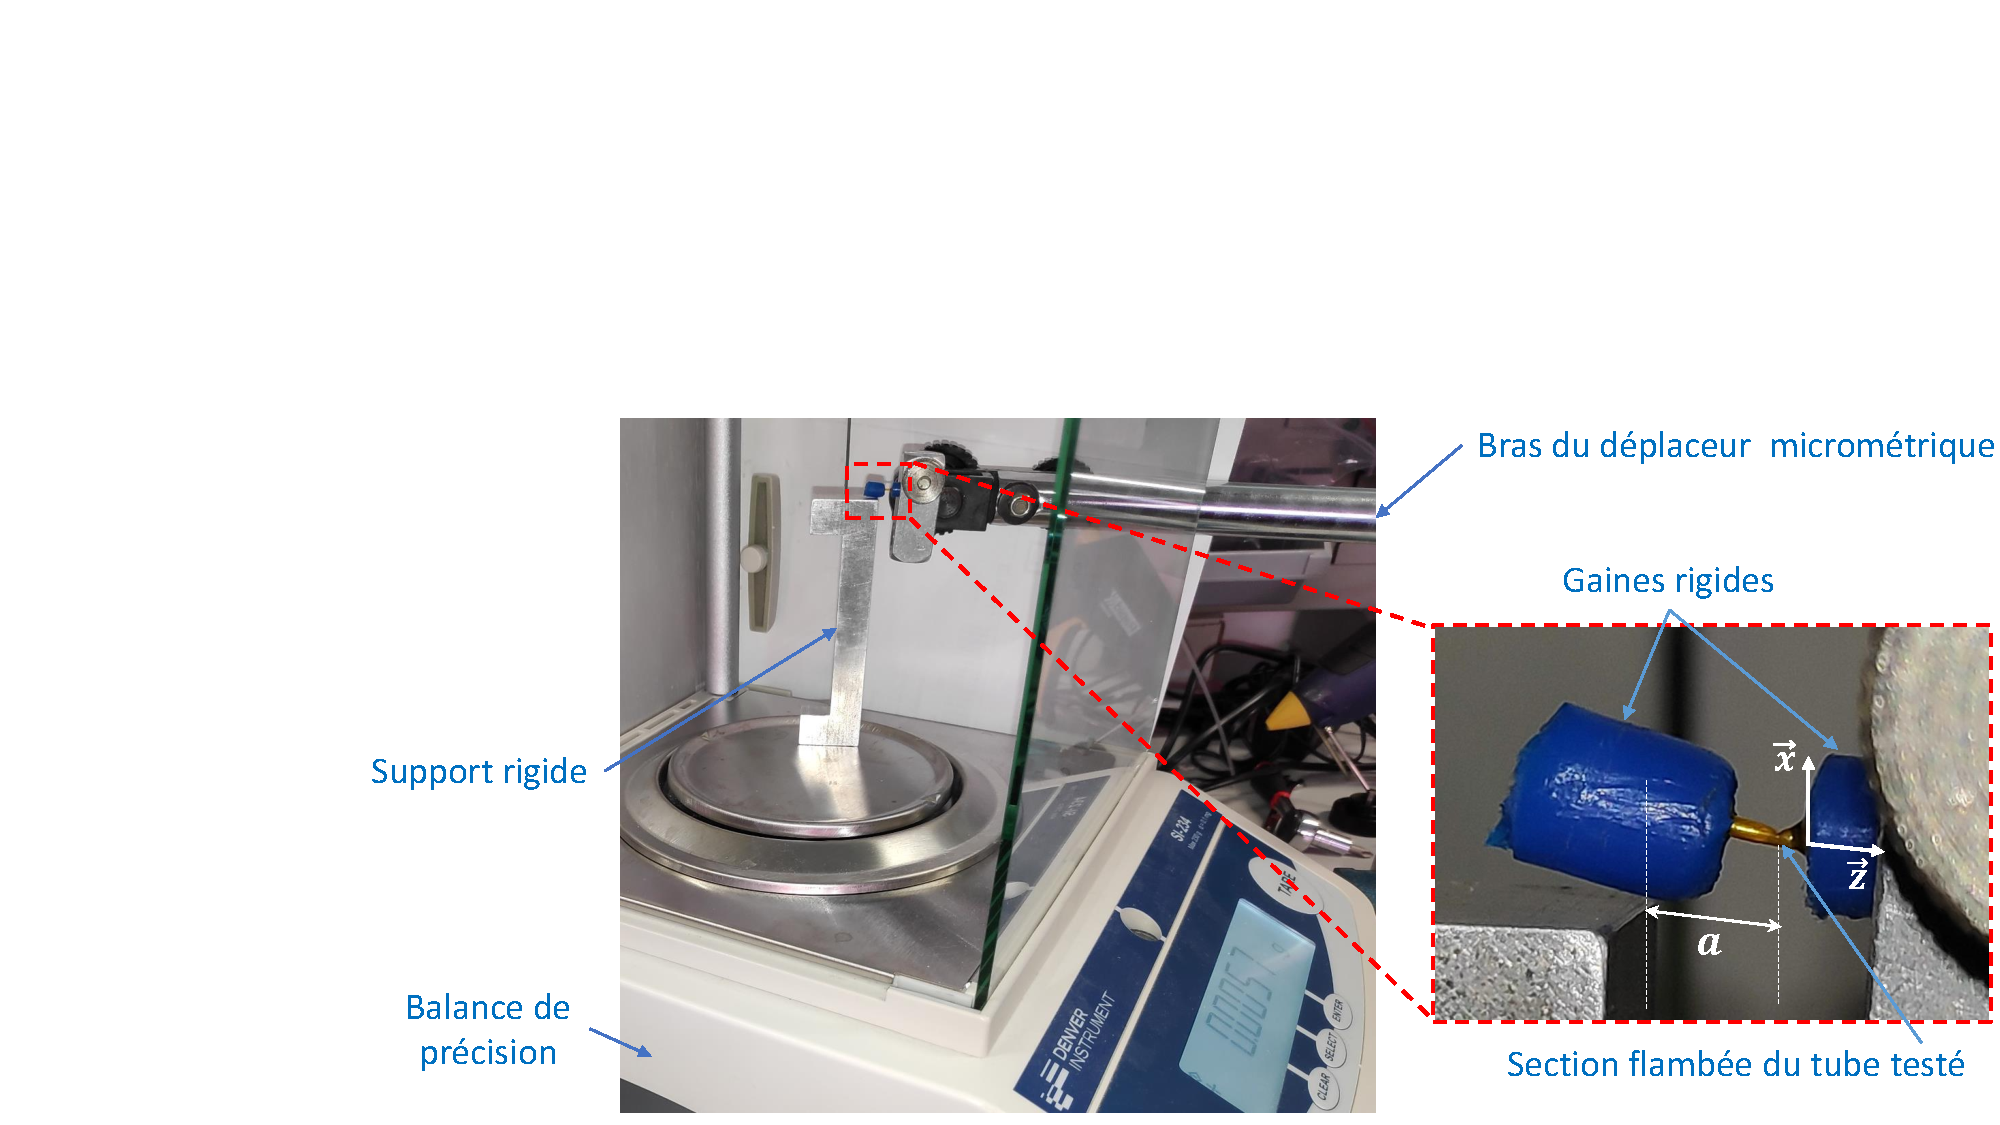
\includegraphics[trim={6cm 0cm 0cm 7cm},clip,width=\textwidth]{../Chap4/Figure/BDT_statique_VH.pdf}
		\caption{Banc d'essai pour la caractérisations statique de tubes en flexion}
		\label{fig:BDT_statique_VH}
	\end{center}
\end{figure}   
%%%%%%%%%%%%%%%%%%%%%%%%%%%%%%%%%%%%     
Le déroulement des essais consiste ensuite à faire descendre le déplaceur micrométrique suivant $\vec{x}$ afin que le tube fléchisse. Lorsque cela se produit, on peut mesurer la distance $a$ qui est le bras de levier de pliage à partir duquel le flambement apparaît sur le tube testé. Les mesures peuvent ainsi commencer après ce premier aller-retour post-flambement permettant d'amorcer l'endroit, sur la longueur du tube, où celui-ci flambera. Cela revient à fixer $a$, et, par extension, le centre de rotation $O$ qui se trouve au centre de la section flambée. La valeur de la masse $m_b$ mesurée sur la balance permet alors de calculer le moment $M_t$ généré par le tube sur le support en aluminium (éq. \ref{eq:Mt_balance}). Une schématisation de la configuration de test, mettant en évidence tous les paramètres de l'essai, est présentée sur la figure \ref{fig:essais_statique_total}.
\begin{equation}
	M_t = \dfrac{m_b\ g\ a}{\cos(\theta)}
	\label{eq:Mt_balance}
\end{equation}
Le terme d'angle qui s'ajoute à l'équation découle du fait que la balance ne mesure que la composante sur l'axe  $\vec{x}$ de la force $\vec{F_t}$, associé au moment $M_t$. Le moment est en effet défini de la même façon que pour le modèle théorique à l'équation \ref{eq:theta=f(x_m)}. La rigidité en rotation $K_t$ du tube testé peut alors être calculée à partir de l'équation \ref{eq:Kt_balance}. On parlera de $K_t$ lors des caractérisations statiques des portions de tubes kapton. Elle est équivalente à la raideur $K_{VH}$ lorsque la VH est fabriquée à partir du tube en question.
 \begin{equation}
	K_t = \dfrac{M_t}{\theta}
	\label{eq:Kt_balance}
\end{equation}
%%%%%%%%%%%%%%%%%%%%%%%%%%%%%%%%%%%%	
\begin{figure}[!htb]
	\begin{center}
		\begin{subfigure}[t]{0.69\textwidth}
			\captionsetup{justification=centering}
			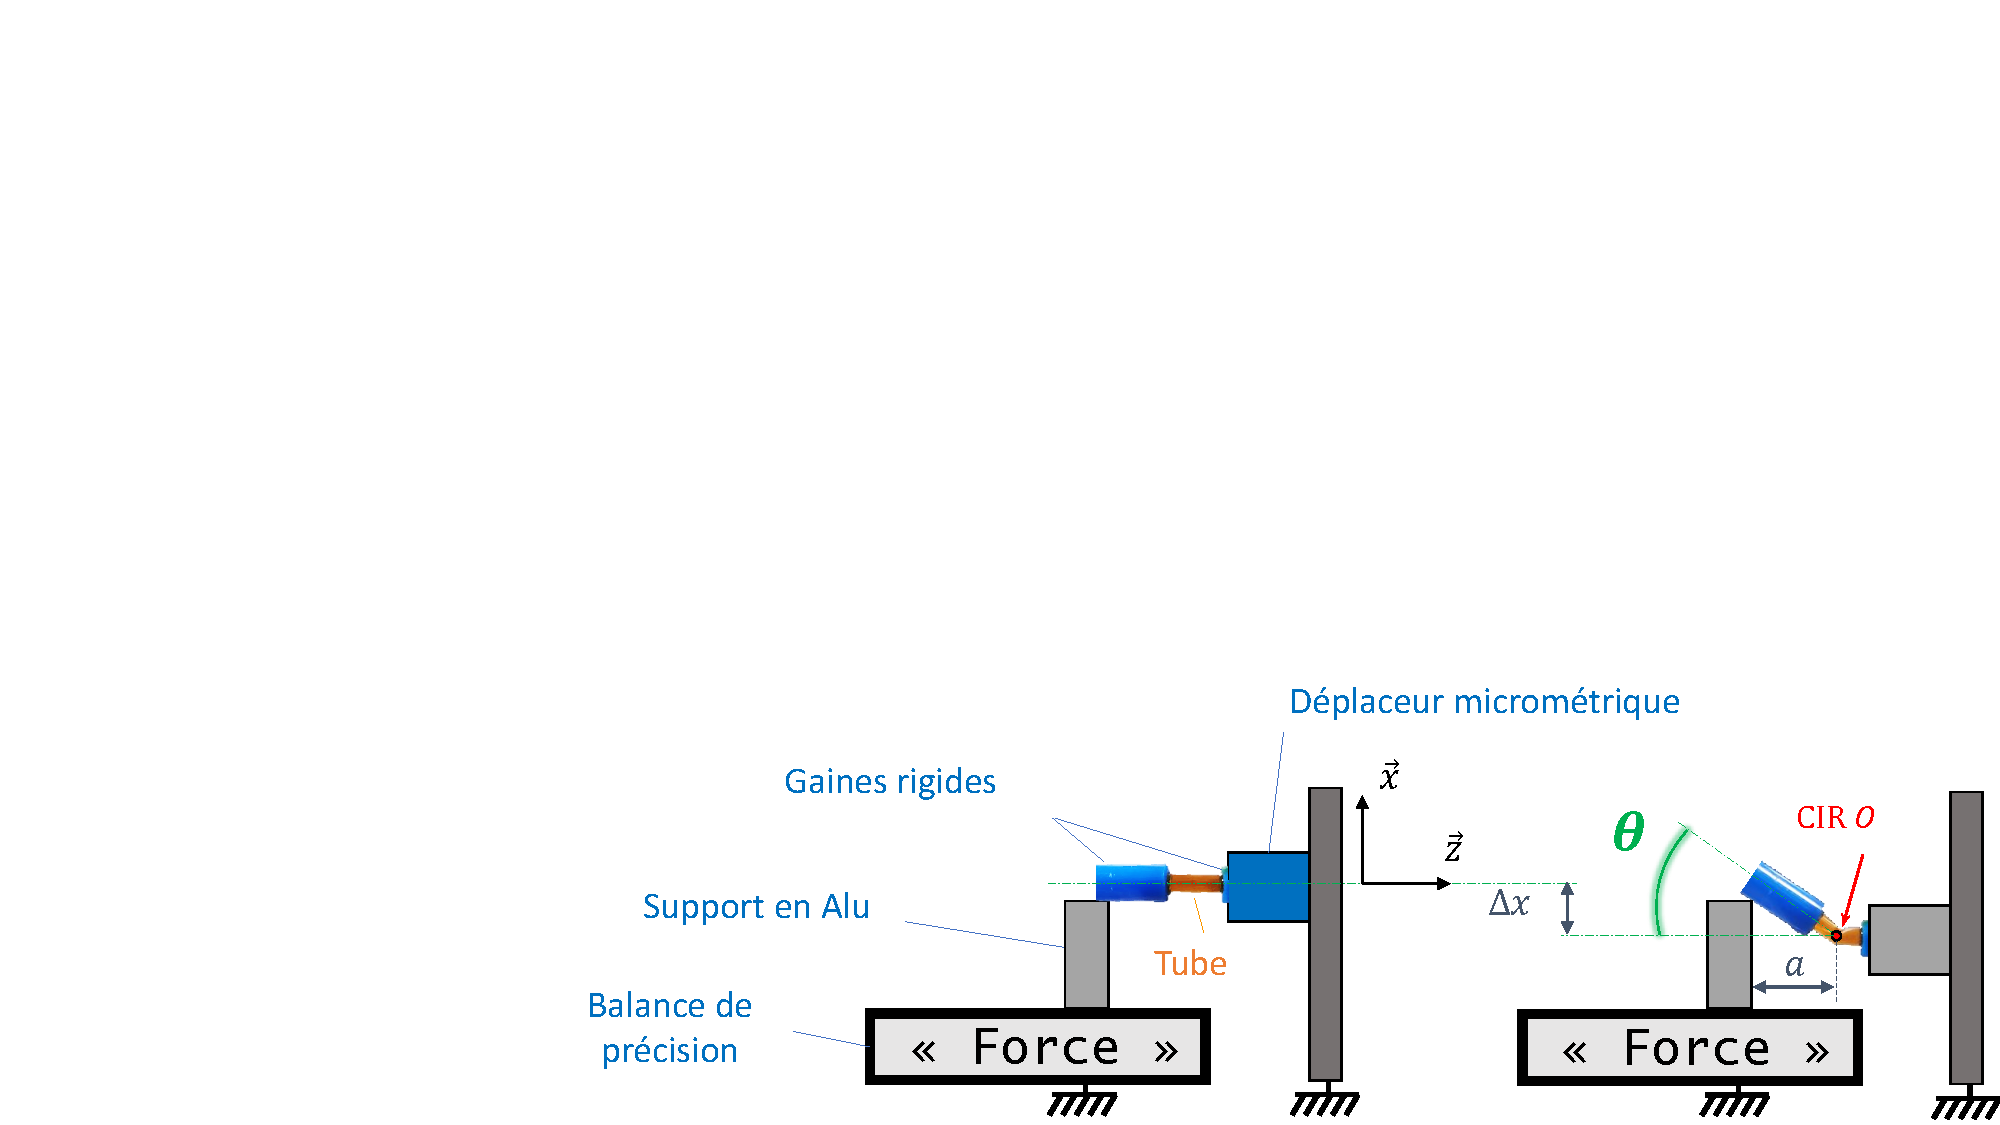
\includegraphics[trim={9.8cm 0cm 0cm 11cm},clip,width=\textwidth]{../Chap4/Figure/essais_statique_VH.pdf}
			\caption{Vue globale}
			\label{fig:essais_statique_VH}
		\end{subfigure}
		\hfillx
		\begin{subfigure}[t]{0.29\textwidth}
			\captionsetup{justification=centering}
			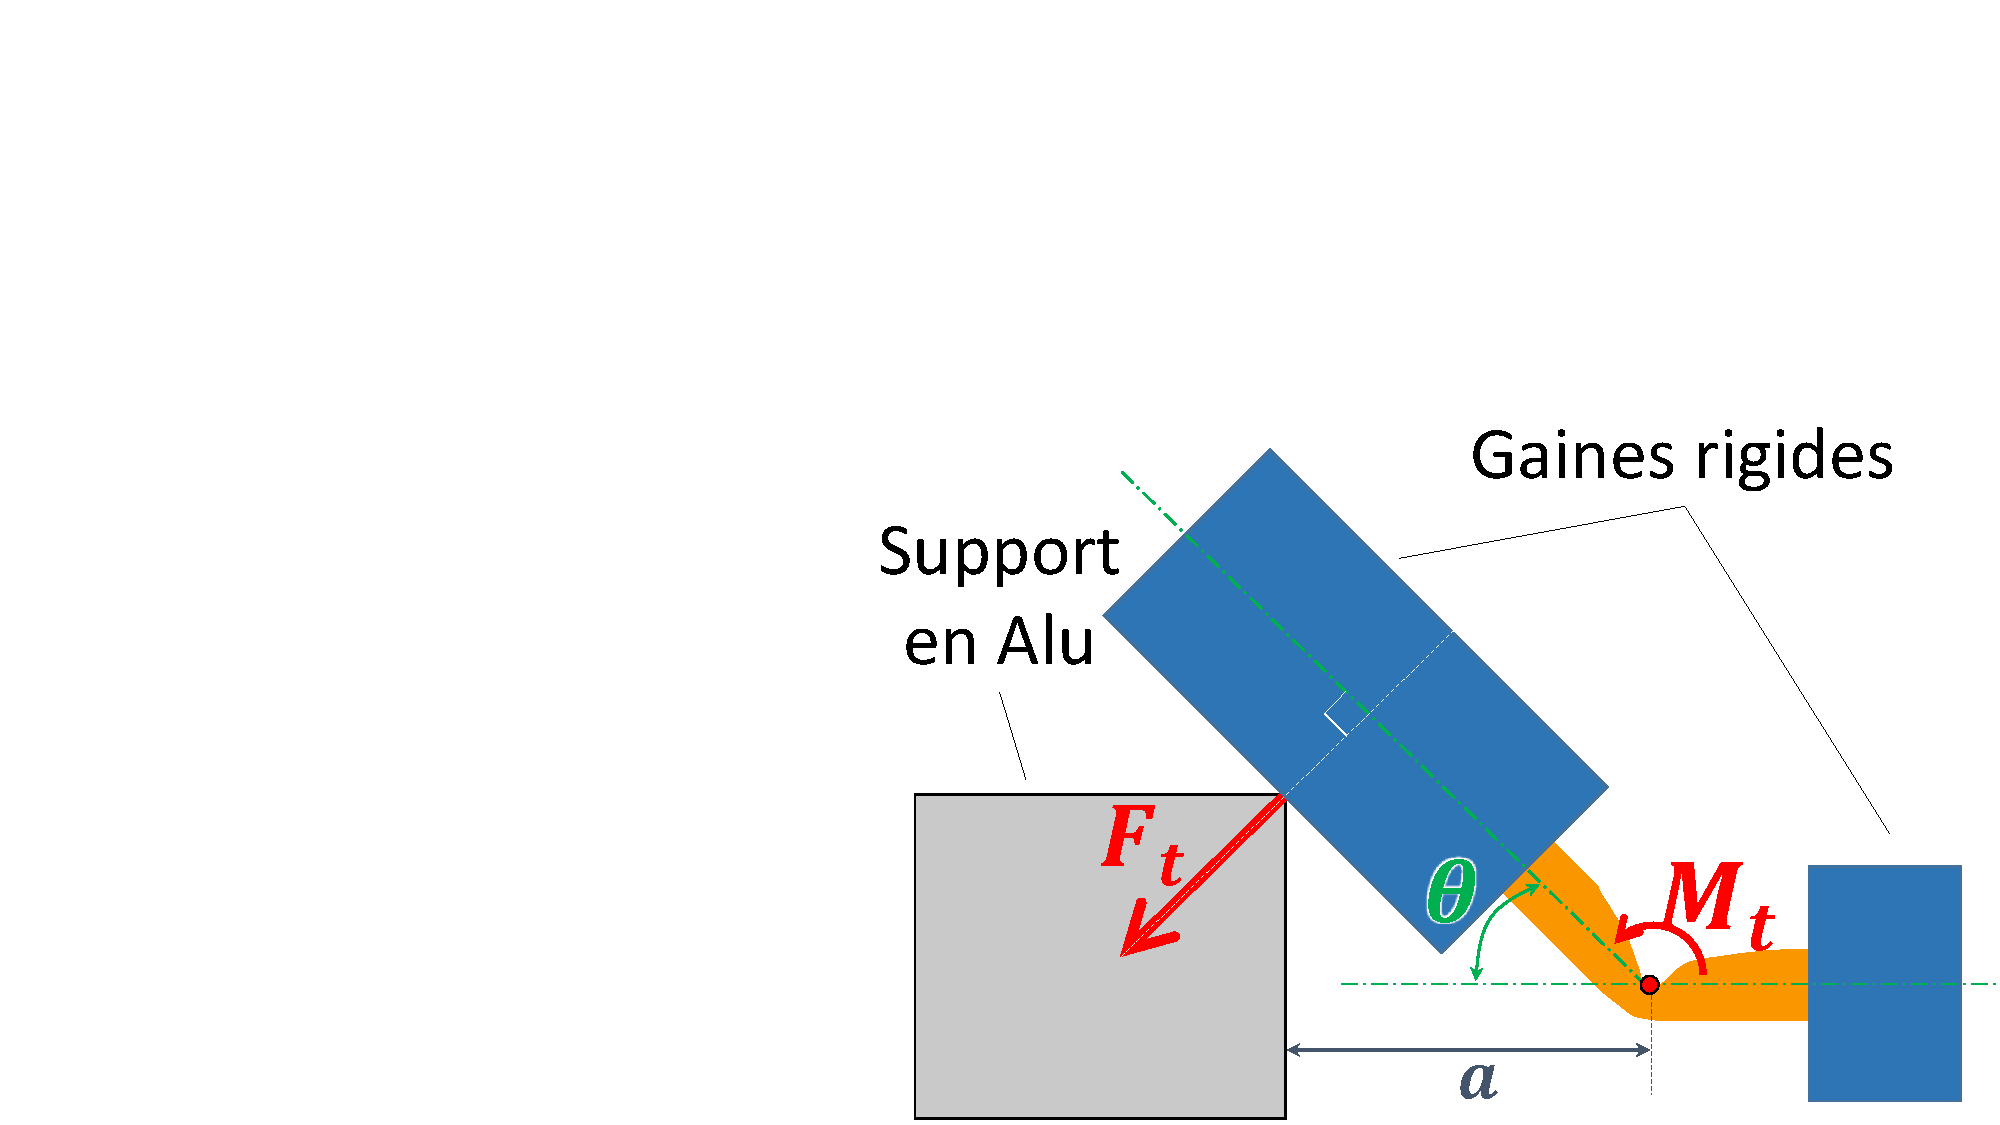
\includegraphics[trim={14cm 0cm 0cm 7cm},clip,width=\textwidth]{../Chap4/Figure/essais_statique_detail.pdf}
			\caption{Détail du contact support-échantillon}
			\label{fig:essais_statique_detail}
		\end{subfigure}
		\caption{Schéma des essais de caractérisations statiques de tubes en flexion}
		\label{fig:essais_statique_total}
	\end{center}
\end{figure}
%%%%%%%%%%%%%%%%%%%%%%%%%%%%%%%%%%%% 
    %///////////////////////////////////////////// 		
	\subsection{Résultats et discussion}
	\label{subsec:4.2.4_Résultats et discussion}
    %/////////////////////////////////////////////	    
Nous avons réalisé les essais statiques sur quatre échantillons de tubes kapton de dimensions différentes qu'on nommera par leurs références T50, T100, T200 et T300. Les dimensions, ainsi que les ratios entre elles, ont été listés dans le tableau \ref{tab:dim_tube_statique}. Les longueurs et diamètres des tubes ont été choisis en accord avec l'encombrement imposé par le contexte applicatif. L'épaisseur des tubes a été prise la plus faible possible afin de limiter la raideur du tube et minimiser l'impact de la plastification locale qui rend plus difficile le retour du tube dans son état initial après flambement.
%%%%%%%%%%%%%%%%%%%%%%%%%%%%%%%%%%%%	
\begin{figure}[!htb]
	\begin{center}
		\captionsetup{justification=centering}
		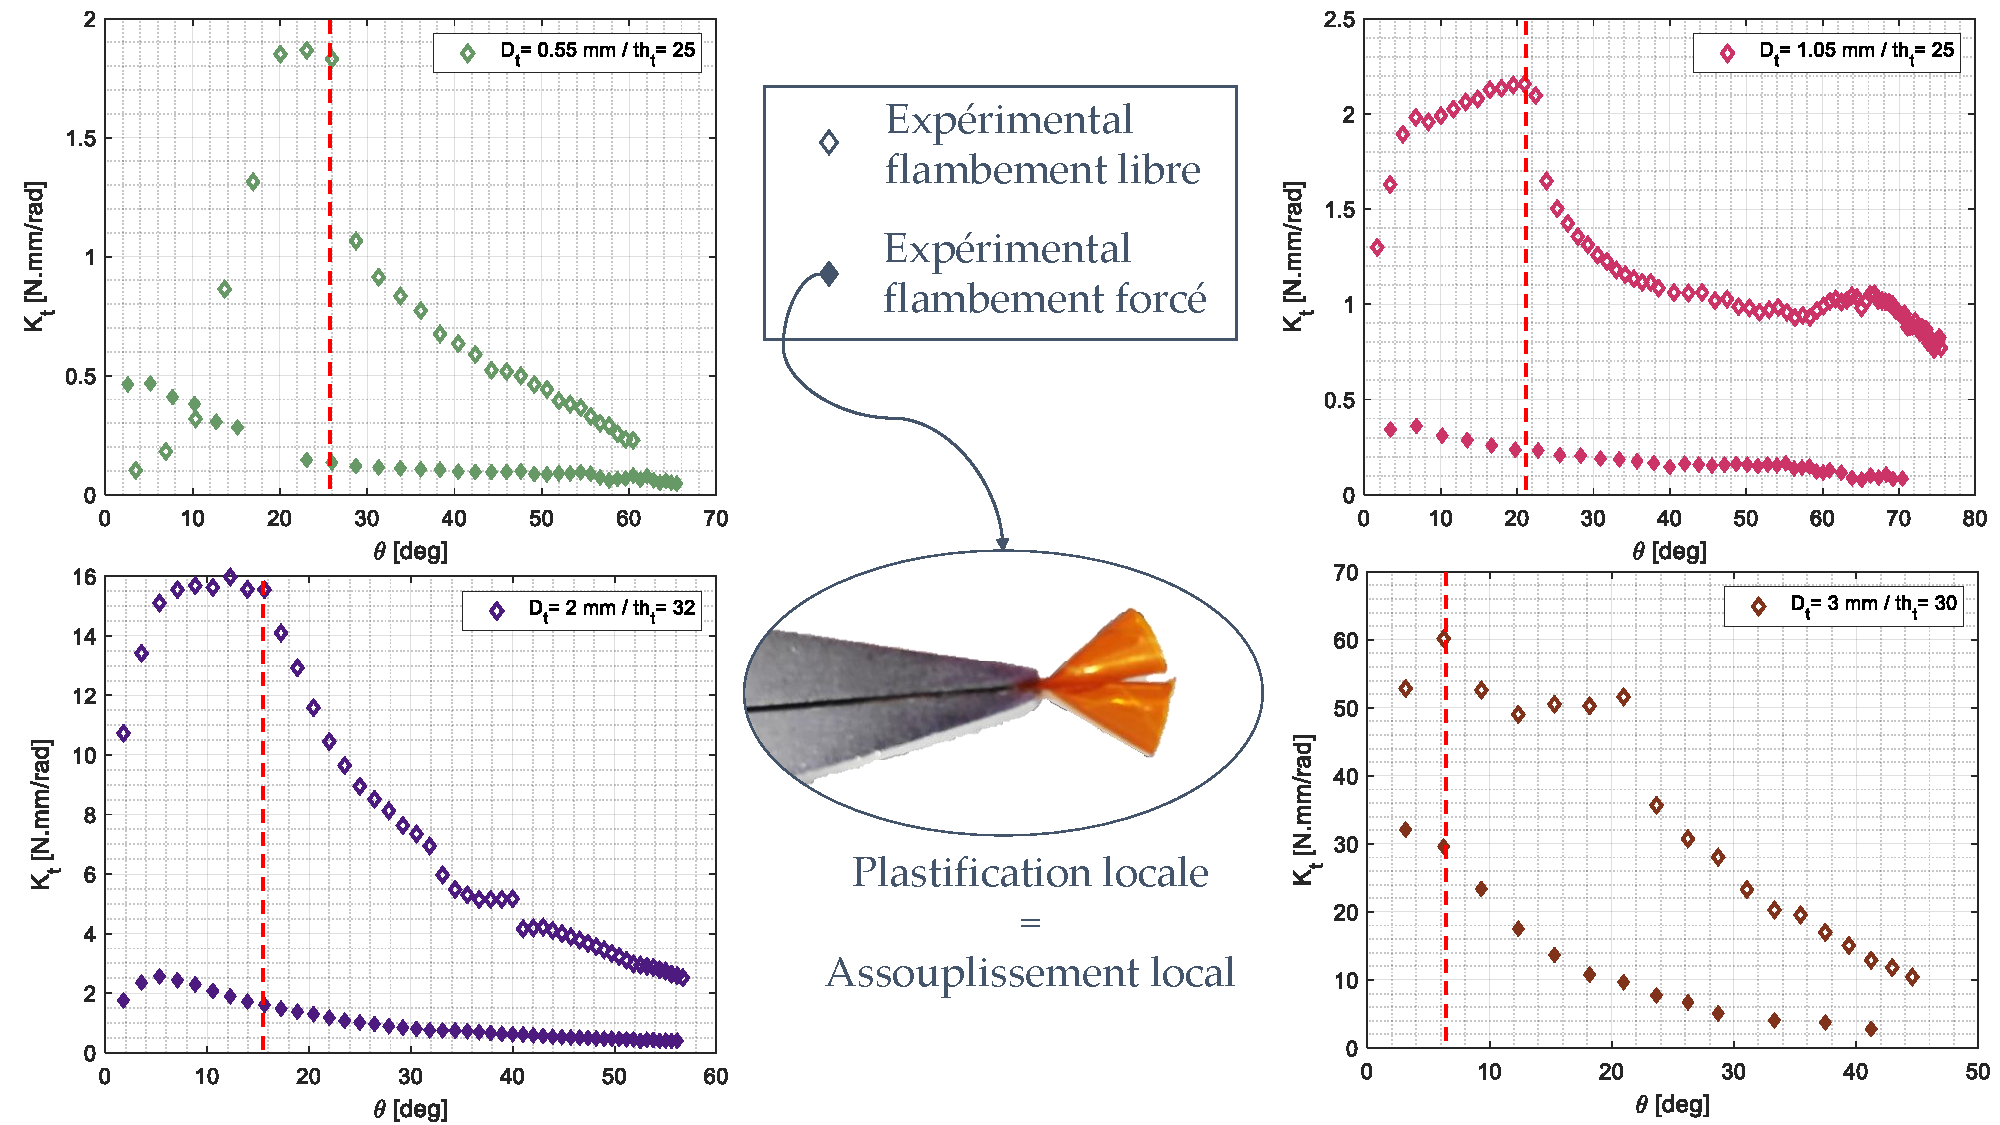
\includegraphics[trim={0cm 0cm 0cm 0cm},clip,width=\textwidth]{../Chap4/Figure/resultats_essais_statique_VH_tous_sans_simu.pdf}
		\caption{Évolutions expérimentales de $K_t$ en fonction de $\theta$ pour quatre tubes de dimensions différentes (tab. \ref{tab:dim_tube_statique})}
		\label{fig:resultats_essais_statique_VH_tous}
	\end{center}
\end{figure} 
%%%%%%%%%%%%%%%%%%%%%%%%%%%%%%%%%%%% 
%%%%%%%%%%%%%%%%%%%%%%%%%%%%%%%%%%%%	
\begin{table}[!htbp]
	\centering
	\captionsetup{justification=centering}
	\rowcolors[]{2}{black!8}{}{
	\begin{tabular}[t]{c||c|c|c|c}
		\toprule
		\rowcolor{blue!10}
		\textbf{Paramètre} & \textbf{T50} & \textbf{T100} & \textbf{T200} & \textbf{T300} \\
		\midrule
		$D_t$ [mm]         & 0.55         & 1.05          & 1.99          & 3             \\	
		$th_t$ [$\micro$m] & 25           & 25            & 32            & 30            \\	
		$L_t$ [mm]         & 1.9          & 3             & 5.8           & 11.1          \\	
		$D_t/th_t$ [ ]     & 22           & 42            & 62            & 100           \\	
		$L_t/D_t$ [ ]      & 3.5          & 3             & 2.9           & 3.7           \\	
		$L_t/th_t$ [ ]     & 76           & 120           & 181           & 370           \\
		\bottomrule
	\end{tabular}}
	\caption{Dimensions des tubes testés sur le banc expérimental statique}
	\label{tab:dim_tube_statique}
\end{table}    
%%%%%%%%%%%%%%%%%%%%%%%%%%%%%%%%%%%%

Sur la figure \ref{fig:resultats_essais_statique_VH_tous} nous pouvons trouver les résultats des essais expérimentaux en marqueurs diamant vide représentant les essais de flambement libre. L'angle de flambement est repéré par un trait rouge vertical sur les essais respectifs. Il est caractérisé par un changement de l'évolution de $K_t$ qui, à partir de ce point, commence à décroître en fonction de $\theta$.

Mis à part pour le tube T100, le flambement semble apparaître pour des angles d'autant plus petits que le rapport $D_t/th_t$ est grand. À partir de son apparition, la décroissance de la raideur en rotation pour tous les tubes devient significative avec l'augmentation de $\theta$. Cette caractéristique remarquable est un atout majeur pour le fonctionnement des VH. Pour minimiser leur raideur, il sera donc préférable de les faire travailler dans une plage d'angle se situant de préférence post-flambement. En ce sens, il faut privilégier un tube dont le rapport $D_t/th_t$ est important pour que l'angle de flambement soit le plus faible possible. Cependant, on voit en comparant les résultats des quatre tubes, que l'ordre de grandeur de la raideur est proportionnel à $D_t$. Il y a donc un compromis à trouver sur les paramètres du tube suivant les critères suivants :
\begin{itemize}[label=$\circ$]
		\item Maximiser $D_t/th_t$ pour minimiser l'angle d'apparition du flambement.
		\item Minimiser $D_t$ pour minimiser $K_t$
\end{itemize}
%%%%%%%%%%%%%%%%%%%%%%%%%%%%%%%%%%%%	
\begin{figure}[!htb]
	\begin{center}
		\captionsetup{justification=centering}
		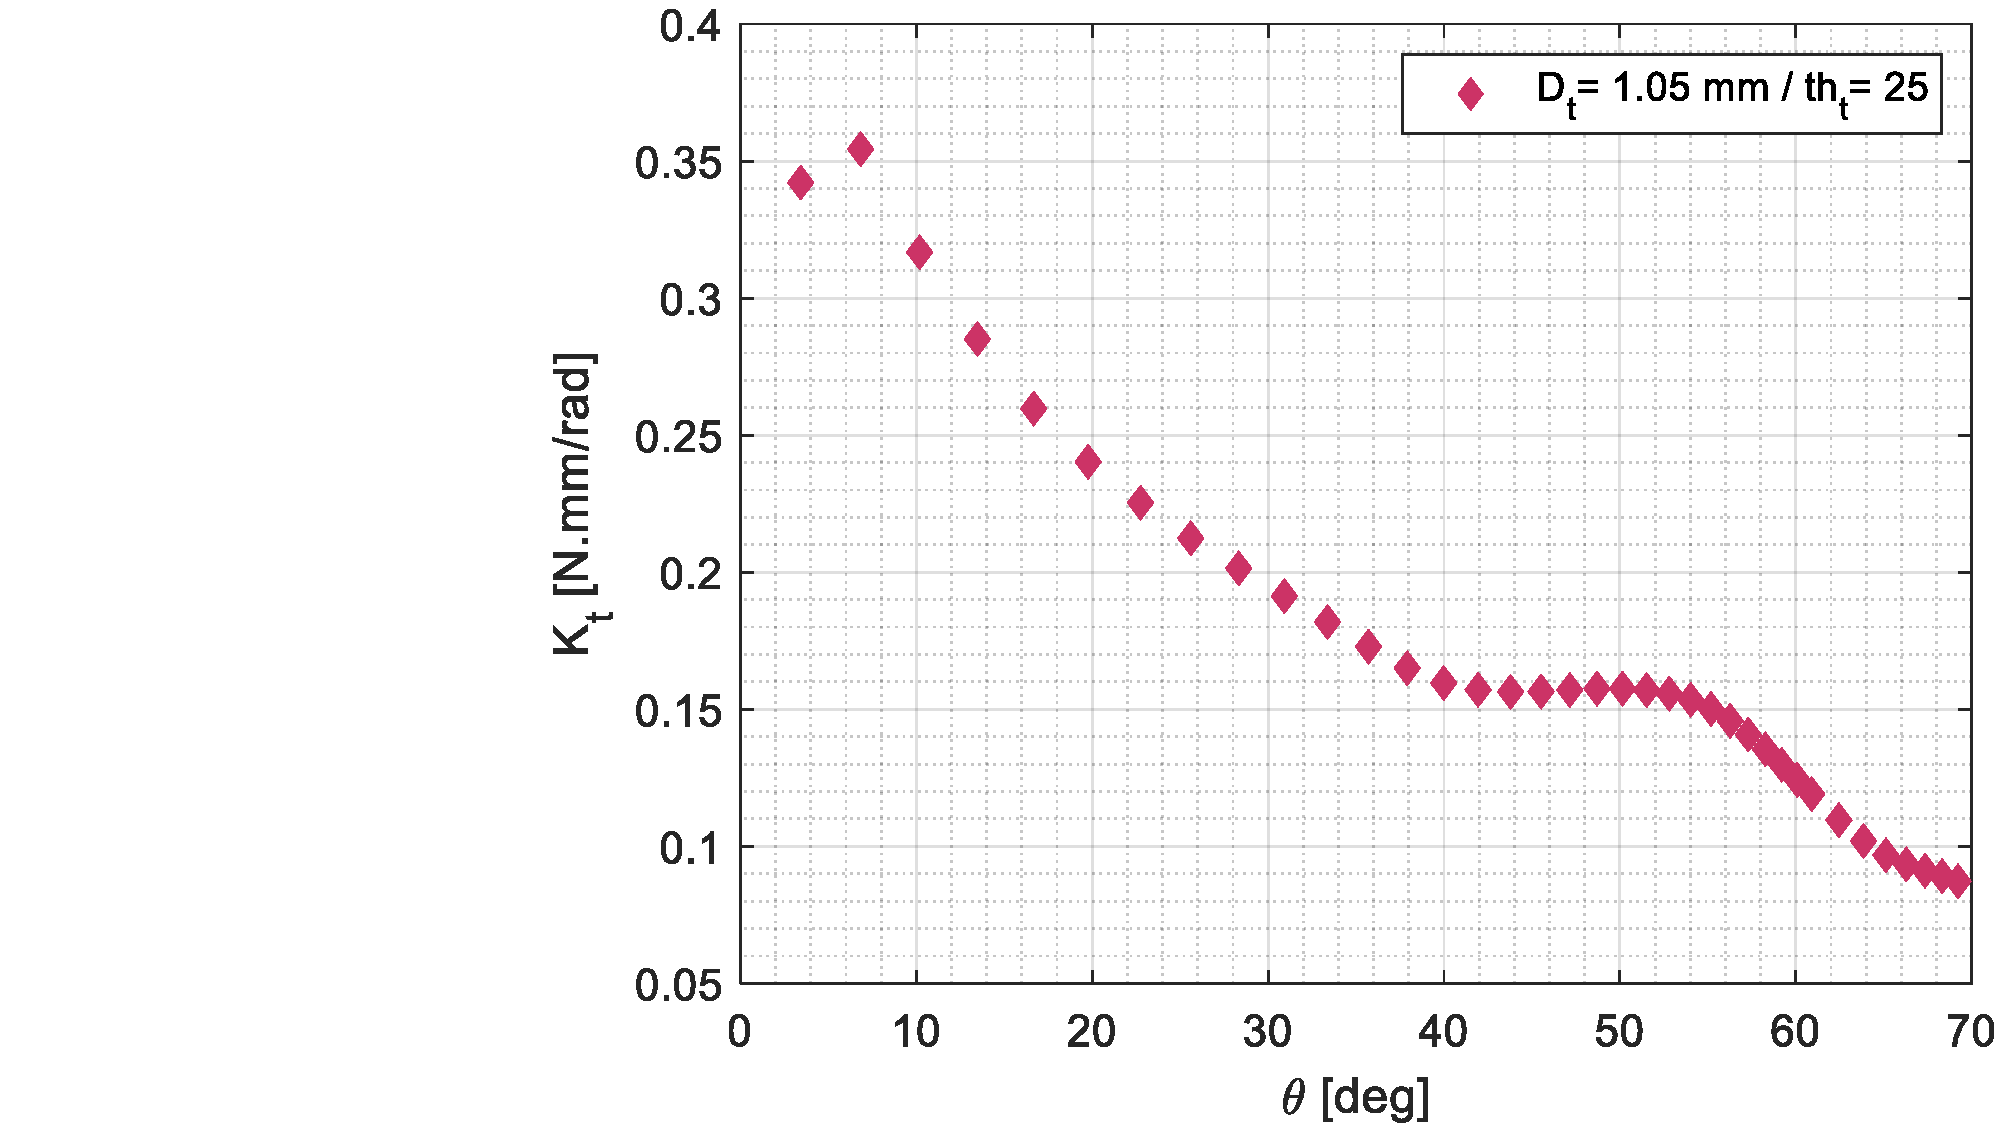
\includegraphics[trim={9.5cm 0cm 0cm 0cm},clip,width=0.6\textwidth]{../Chap4/Figure/(K_VH)_vs_theta_D1mm_plastifie_essai2.pdf}
		\caption{Évolution de $K_t$ en fonction de $\theta$ pour le tube T100 plastifié}
		\label{fig:(K_VH)_vs_theta_D1mm_plastifie}
	\end{center}
\end{figure}    
%%%%%%%%%%%%%%%%%%%%%%%%%%%%%%%%%%%% 
En regardant l'ordre de grandeur des valeurs admissibles pour $K_{VH}$ (fig. \ref{fig:(K_VH)_max(a)_et_Deltatheta_pour_bistabilite}), on peut dire que les tubes T50 et T100 sont théoriquement les deux choix à privilégier sur les quatre tubes testés. En considérant l'assouplissement des LFs, la raideur du tube T100 se retrouve à la limite de l'admissibilité. Une solution à ce problème a été trouvée en pré-plastifiant localement l'articulation à la section flambée afin de l'assouplir. Les marqueurs diamants pleins sur la figure \ref{fig:resultats_essais_statique_VH_tous} montrent les résultats des essais statiques réalisés sur les quatre échantillons précédents après leur plastification locale. On nommera alors respectivement T50p, T100p, T200p et T300p les tubes résultants avec les caractéristiques mécaniques modifiées. La raideur en rotation baisse alors significativement pour tous les tubes plastifiés. 
%%%%%%%%%%%%%%%%%%%%%%%%%%%%%%%%%%%%	
\begin{figure}[!htb]
	\begin{center}
		\captionsetup{justification=centering}
		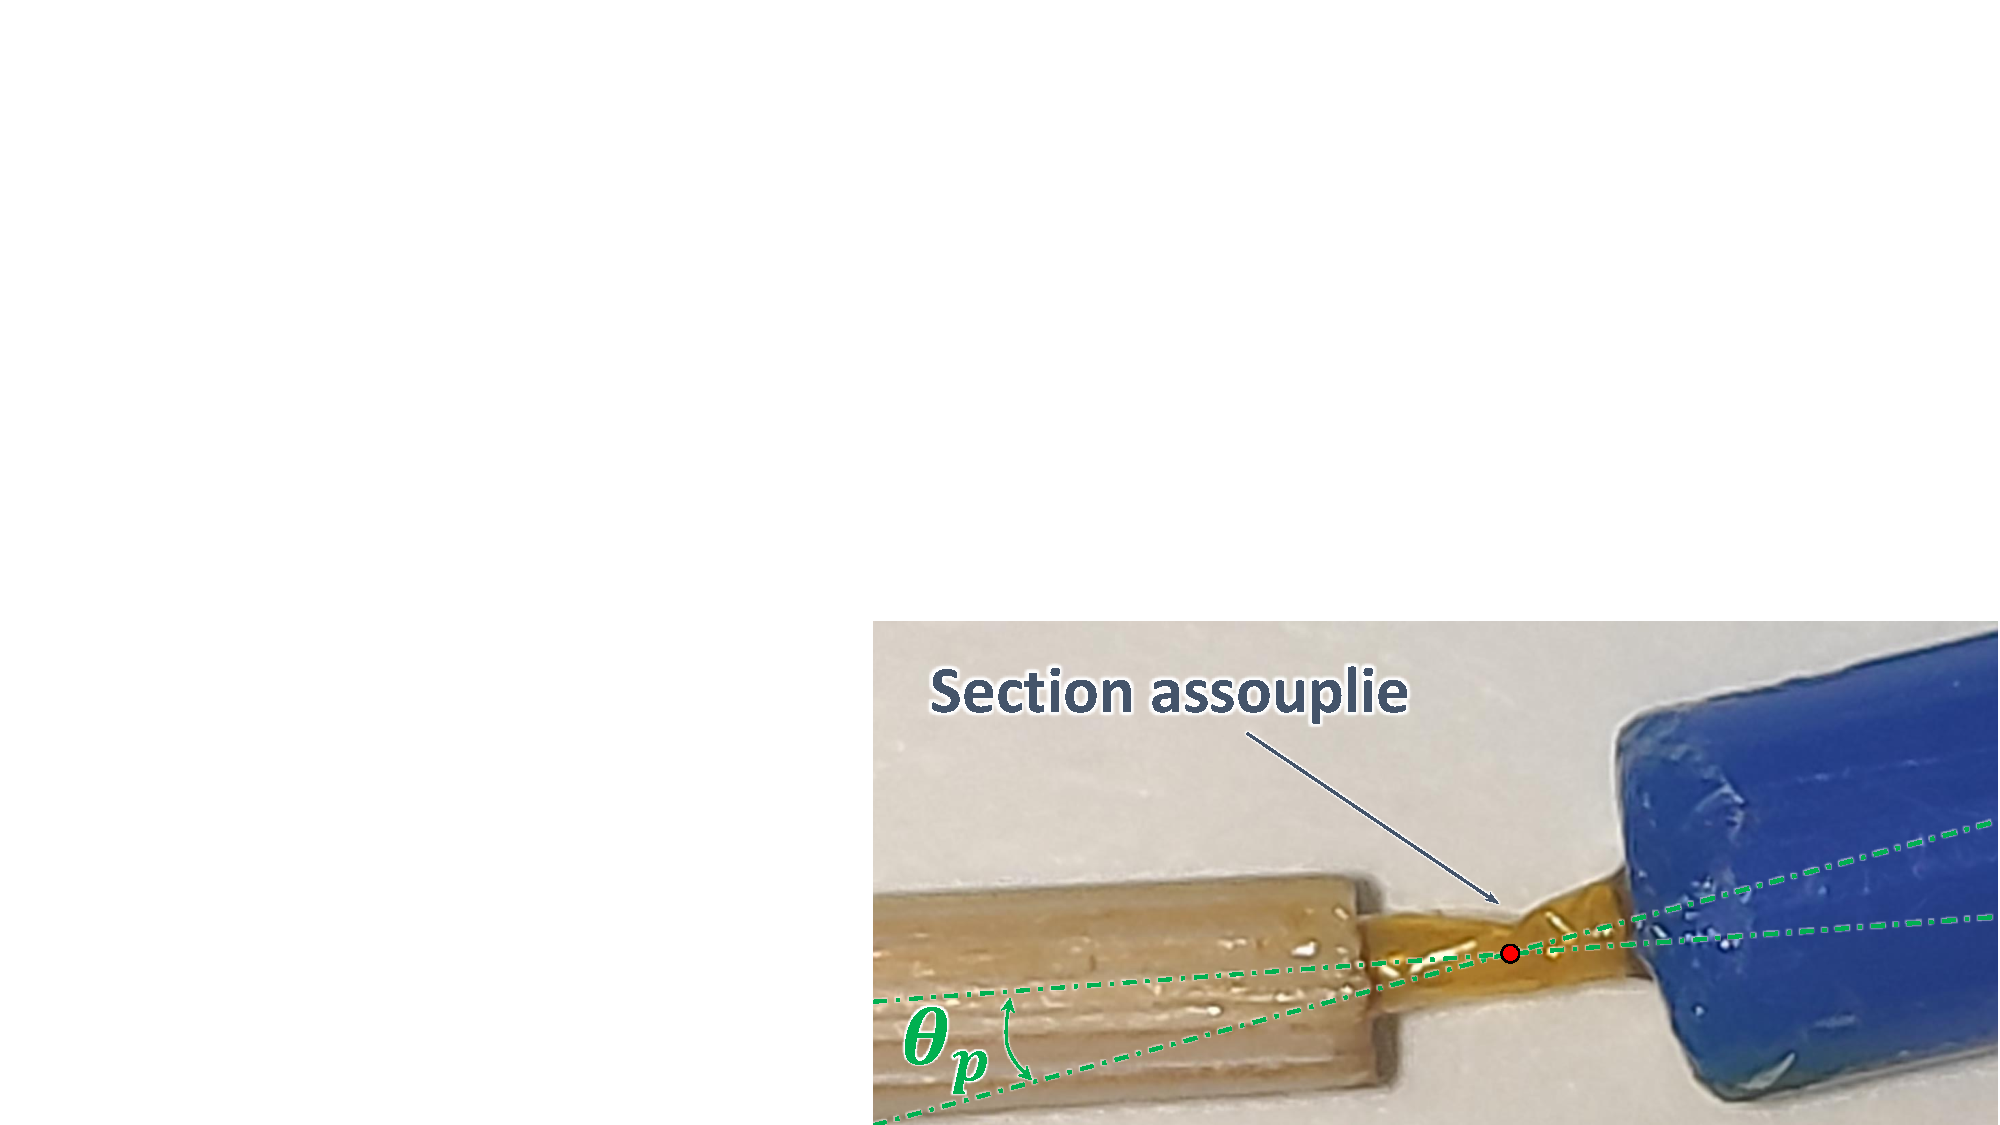
\includegraphics[trim={15cm 0cm 0cm 11cm},clip,width=0.4\textwidth]{../Chap4/Figure/plastification_tube.pdf}
		\caption{Image du tube T100 plastifié}
		\label{fig:plastification_tube}
	\end{center}
\end{figure}
%%%%%%%%%%%%%%%%%%%%%%%%%%%%%%%%%%%% 

Le pincement local ne doit pas compromettre l'étanchéité du tube. On réalise alors un essai expérimental consistant à obstruer une extrémité du tube plastifié et imposer une pression de fluide de l'ordre de 50kPa à l'autre extrémité. Cette pression est 10 fois supérieure à la pression de fonctionnement et n'induit aucune fuite. La figure \ref{fig:(K_VH)_vs_theta_D1mm_plastifie} montre le tube T100p après un essai statique. Un angle $\theta_p$ estimé à \ang{5} est alors induit suite à la déformation par pincement, mais la section de passage semble néanmoins intacte, au point de rotation, sur le tube en repos. L'influence de cet angle sera à prendre en considération pour les essais de caractérisations hydrauliques. Sur les deux candidats envisageables, nous choisissons de continuer avec le T100p, car ses dimensions le rendent plus manipulable que le tube T50p. La figure \ref{fig:(K_VH)_vs_theta_D1mm_plastifie} montre alors un focus sur les résultats des essais statiques réalisés sur le tube T100p. 

Il faut à présent déterminer si les pertes de charges générées au travers du tube T100p flambé remplissent le critère hydraulique du cahier des charges d'une VH.     
%/!\/!\/!\/!\/!\/!\/!\/!\/!\/!\/!\/!\/!\/!\/!\/!\/!\/!\/!\/!\/!\/!\/!\/!\ 		
\section{Caractérisation expérimentale du comportement hydraulique d'une VH}
\label{sec:4.4_Caractérisations hydrauliques}
%/!\/!\/!\/!\/!\/!\/!\/!\/!\/!\/!\/!\/!\/!\/!\/!\/!\/!\/!\/!\/!\/!\/!\/!\ 	
Nous avons vu, par l'équation \ref{eq:Cf_definition}, que les PdC engendrées au travers d'une perturbation géométrique dans une conduite dépendent du produit de $Cf$ par le carré du débit de l'écoulement. $Cf$ est une fonction entièrement dépendante de la géométrie de la conduite et des propriétés du fluide. 

Plusieurs choix de fluides incompressibles sont possibles pour remplir le circuit hydraulique. L'eau, les huiles synthétiques, les huiles minérales ou les huiles végétales. L'eau a été écartée pour prévenir une corrosion prématurée des composants hydrauliques. En plus de cet inconvénient, les huiles synthétiques et minérales peuvent contenir des composants toxiques pour la santé. L'huile végétale de tournesol a donc été sélectionnée comme fluide pour les essais hydrauliques. 
Sa masse volumique est de $\rho_{to} = 900$kg/m$^3$, et sa viscosité dynamique est de $\mu_{to}=0.062$Pa.s.

L'inconnue reste alors l'évolution de la section flambée en fonction de l'angle de flexion du tube. Nous allons donc estimer expérimentalement l'évolution de $Cf$ en fonction de $\theta$, pour le tube T100p.
    %/////////////////////////////////////////////	
	\subsection{Présentation du banc de test}
	\label{subsec:4.4.1_Présentation du banc de test}    
    %/////////////////////////////////////////////	
Nous avons conclu, d'après les essais expérimentaux statiques, que le tube T100p, dont les dimensions avant plastification sont données dans le tableau \ref{tab:dim_tube_statique}, est un bon candidat sur le plan mécanique pour l'implémentation sur l'OB. Il s'agit à présent d'étudier son comportement du point de vue hydraulique. Nous allons en ce sens chercher à quantifier le coefficient de PdC sur ce tube et vérifier si son évolution est conforme aux besoins du système de VH qu'on recherche. La conception du banc expérimental pour sa caractérisation hydraulique est illustrée sur la figure \ref{fig:BDT_hydraulique_VH}. Pour faciliter la visibilité, nous avons caché un certain nombre de pièces servant à la mise et au maintien en position sur la vue en perspective de cette conception. Avec le banc d'essai hydraulique, nous recherchons à quantifier les pertes de charges au travers d'un tube flexible, fléchi à un angle $\theta$ donné, dans les conditions cinématiques se rapprochant au mieux de celles de la VH en fonctionnement sur l'OB.

Un plateau tournant motorisé a été conçu pour accueillir un échantillon de tube à caractériser. La partie fixe de celui-ci vient se placer dans le mors cylindrique qui le maintient en position une fois serré, le privant ainsi de tout degré de liberté. Le bras rotatif accueille quant à lui la partie mobile qui sera soumise à des incréments d'angle $\theta$ par rapport à la partie fixe. Ce bras est relié, au travers d'un axe de transmission, à un servomoteur interfacé et commandé sous LabVIEW. Nous pouvons avoir un réglage précis de l'angle, en position statique, mais aussi lui imposer une variation dynamique. En effet, ce banc a été conçu pour reproduire les mouvements de la masse avec une commande analogique en entrée du servomoteur. Néanmoins, dans ce chapitre, il s'agira uniquement de caractériser la VH en position statique pour un angle de flexion donné.
%%%%%%%%%%%%%%%%%%%%%%%%%%%%%%%%%%%%	
\begin{figure}[!htb]
\begin{center}
    \captionsetup{justification=centering} 
	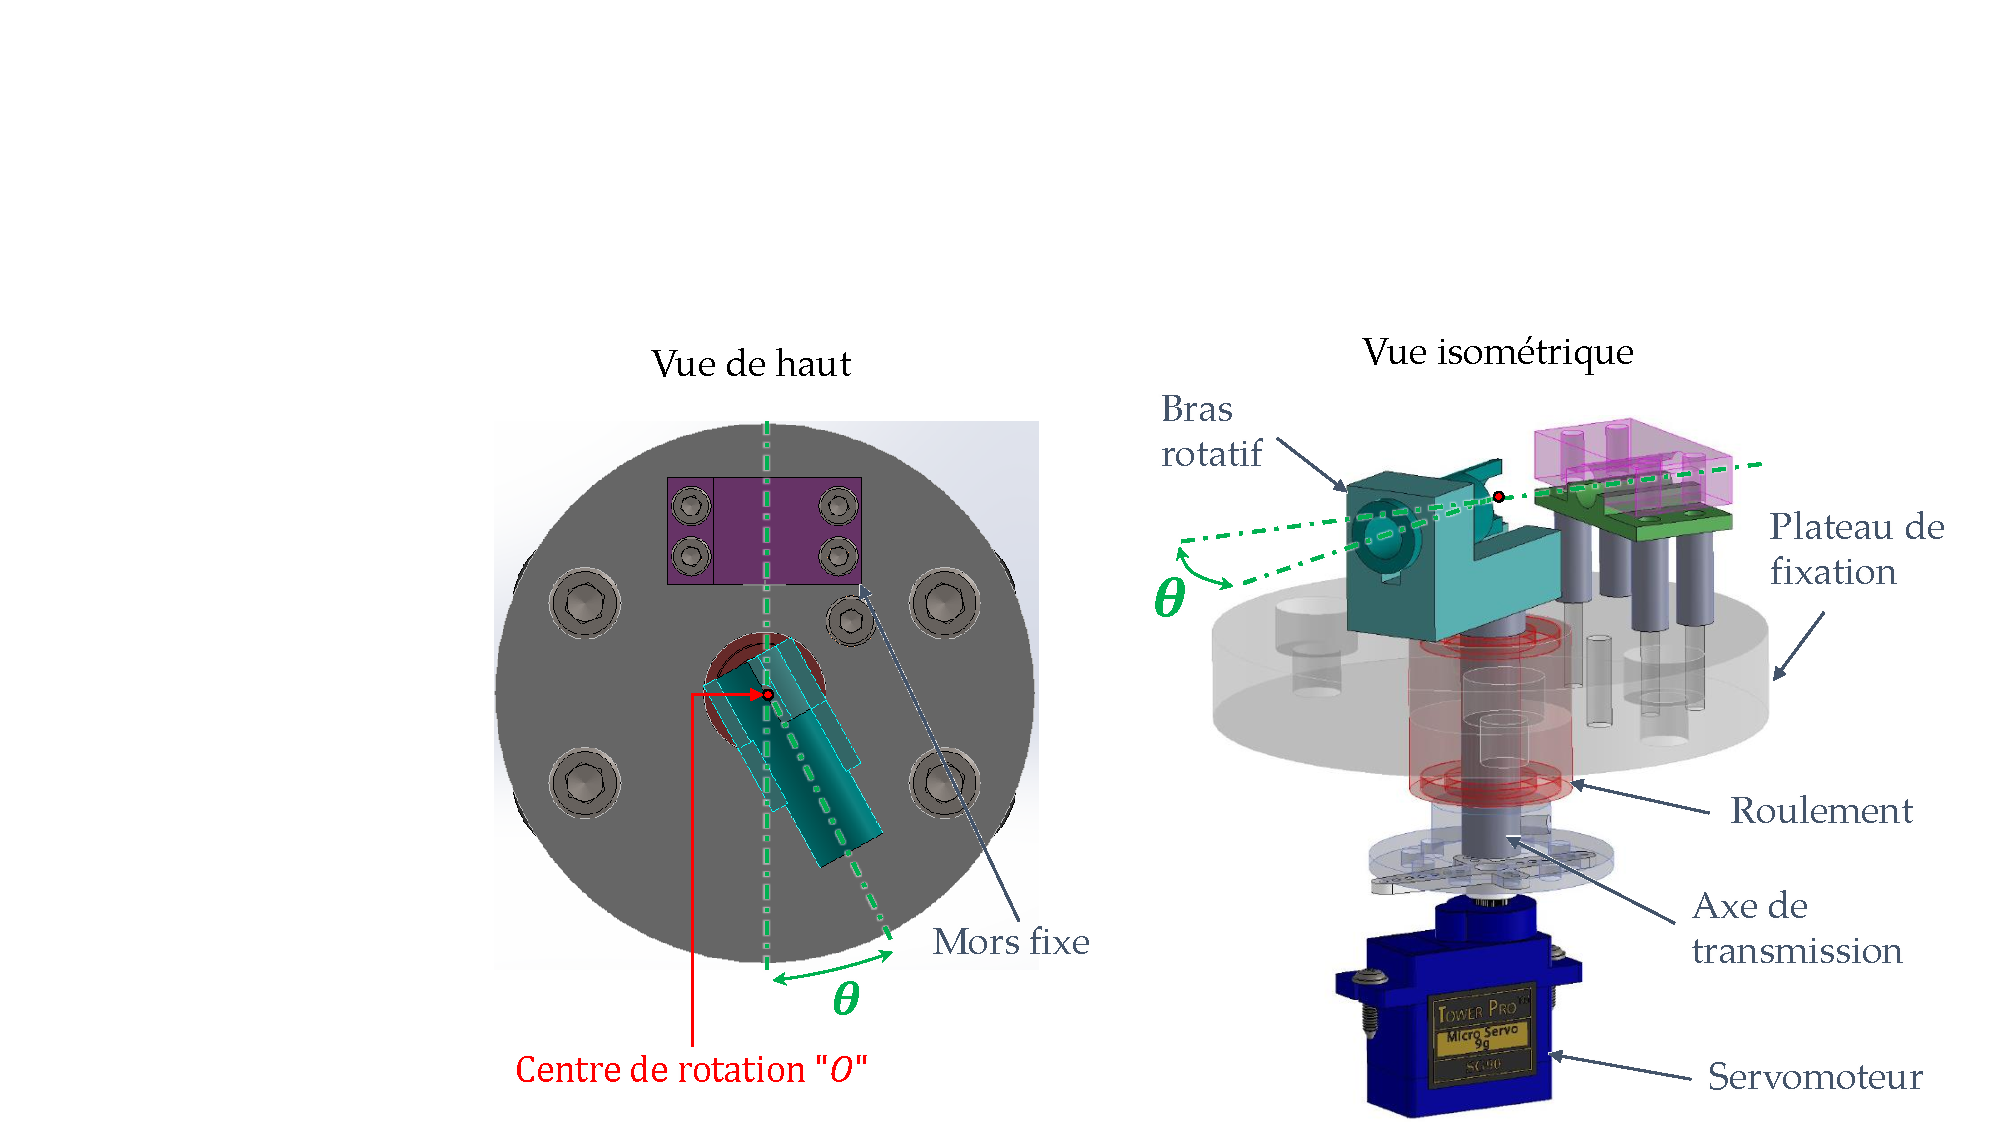
\includegraphics[trim={8cm 0cm 0cm 5cm},clip,width=\textwidth]{../Chap4/Figure/BDT_hydraulique_VH.pdf}
	\caption{Banc d'essai pour la caractérisations hydrauliques de VH}
	\label{fig:BDT_hydraulique_VH}
\end{center}	
\end{figure}    
%%%%%%%%%%%%%%%%%%%%%%%%%%%%%%%%%%%% 

Les schémas des essais hydrauliques sont illustrés sur la figure \ref{fig:essais_hydraulique_VH}. On peut y apercevoir le tube T100p installé sur le plateau rotatif, ainsi que le schéma hydraulique des expériences avec les composants de mesure environnants. Le protocole d'essais consiste à créer un écoulement de fluide à travers la VH en mesurant la pression en amont et en aval de cette dernière. L'écoulement est généré par la vidange d'une seringue dont le déplacement du piston est mesuré par un capteur laser afin de remonter au débit de l'écoulement en connaissant les dimensions de la seringue. Deux capteurs de pression piézorésistifs permettent la mesure de pression amont/aval de la VH et le plateau rotatif permet d'imposer l'angle $\theta$ à chaque vidange.

Les acquisitions sont faites au travers de la même carte NI6212 utilisée dans le chapitre précédent pour la caractérisation expérimentale de l'OB. Les données brutes sont stockées sous LabVIEW au passage d'un buffer s'assurant que tous les points de mesure transmis par les capteurs sont traités par le programme d'acquisition. La carte d'acquisition permet aussi de générer des signaux analogiques et numériques et donc on peut contrôler le servomoteur via le même programme. Un circuit de purge est aussi mis en place afin de chasser l'air du circuit avant le début des essais.
%%%%%%%%%%%%%%%%%%%%%%%%%%%%%%%%%%%%	
\begin{figure}[!htb]
\begin{center}
    \captionsetup{justification=centering} 
	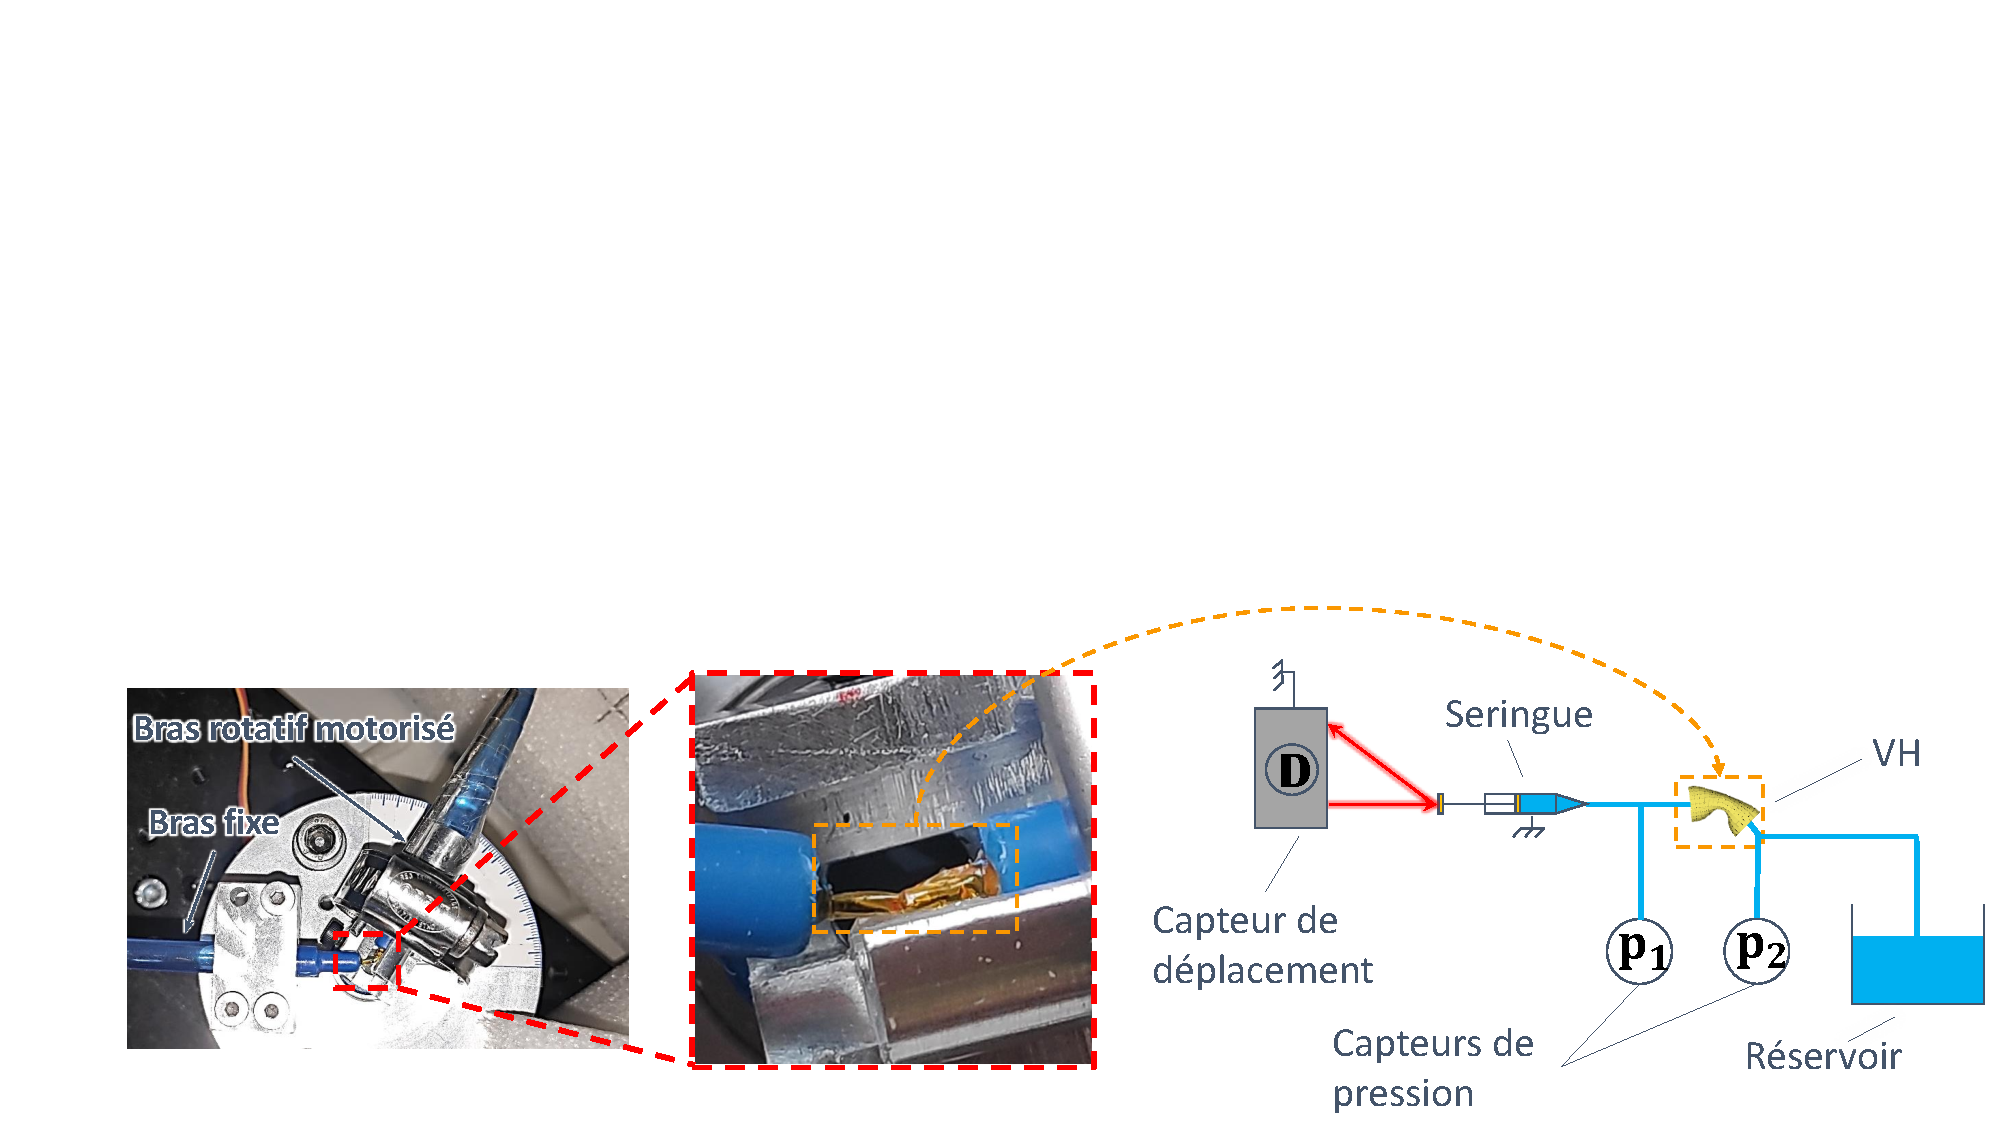
\includegraphics[trim={2cm 0cm 0cm 10cm},clip,width=\textwidth]{../Chap4/Figure/essais_hydraulique_VH.pdf}
	\caption{Essais de caractérisations hydrauliques de VH}
	\label{fig:essais_hydraulique_VH}
\end{center}	
\end{figure}    
%%%%%%%%%%%%%%%%%%%%%%%%%%%%%%%%%%%%  

Le détail de la fabrication de la valve est schématisé sur la figure \ref{fig:fabrication_tube_experimental}. L'échantillon de tube kapton de diamètre $D_t$ est relié de part et d'autre à un morceau de gaine rigide de diamètre $D_{gr}$ qui lui-même s'imbrique à l'intérieur du circuit hydraulique de diamètre $D$ équivalent à celui des pistons. Le diamètre $D_h$ correspond alors au diamètre hydraulique à la section flambée. Cette complexité de fabrication est dû à la souplesse du matériau à manipuler. Idéalement, pour extraire le comportement de la VH seule, il faudrait se munir d'un circuit hydraulique droit et exclusivement composé de tubes de même diamètre afin d'éliminer toute singularité géométrique. Cependant, le circuit hydraulique a été pensé afin de s'adapter aux pistons et donc il aura fallu adapter la VH au circuit hydraulique. En conséquence, les PdC $\Delta p = p_1 - p_2$ mesurées seront une combinaison des PdC $\Delta p_{(c+e)}$ dans les deux contractions brusques et les deux élargissements brusques, et des PdC de la VH.  Ces dernières s'expriment alors par l'équation \ref{eq:DeltaP_VH_exp}. 
\begin{equation}
	\begin{split} 
\Delta p_{VH} & = (p_1 - p_2) - (\Delta p_{c1}+\Delta p_{c2}+\ \Delta p_{e1}+\Delta p_{e2})	\\
			  & = (p_1 - p_2) - \Delta p_{(c+e)}
	\end{split}
	\label{eq:DeltaP_VH_exp}
\end{equation}
$Cf_{VH}$ s'exprime alors avec l'équation \ref{eq:Cf_VH_exp}.
\begin{equation}
	Cf_{VH} = \dfrac{(p_1 - p_2)}{{q_{ser}}^2} - Cf_{(c+e)}
\label{eq:Cf_VH_exp}
\end{equation}
Où $Cf_{(c+e)}$ est le coefficient de PdC induit par les singularités géométriques créées lors de la fabrication. Ce-dernier est quantifié avec un écoulement à $\theta = \ang{0}$, car alors $Cf_{VH}=0$. 
%%%%%%%%%%%%%%%%%%%%%%%%%%%%%%%%%%%%	
\begin{figure}[!htb]
\begin{center}
    \captionsetup{justification=centering} 
	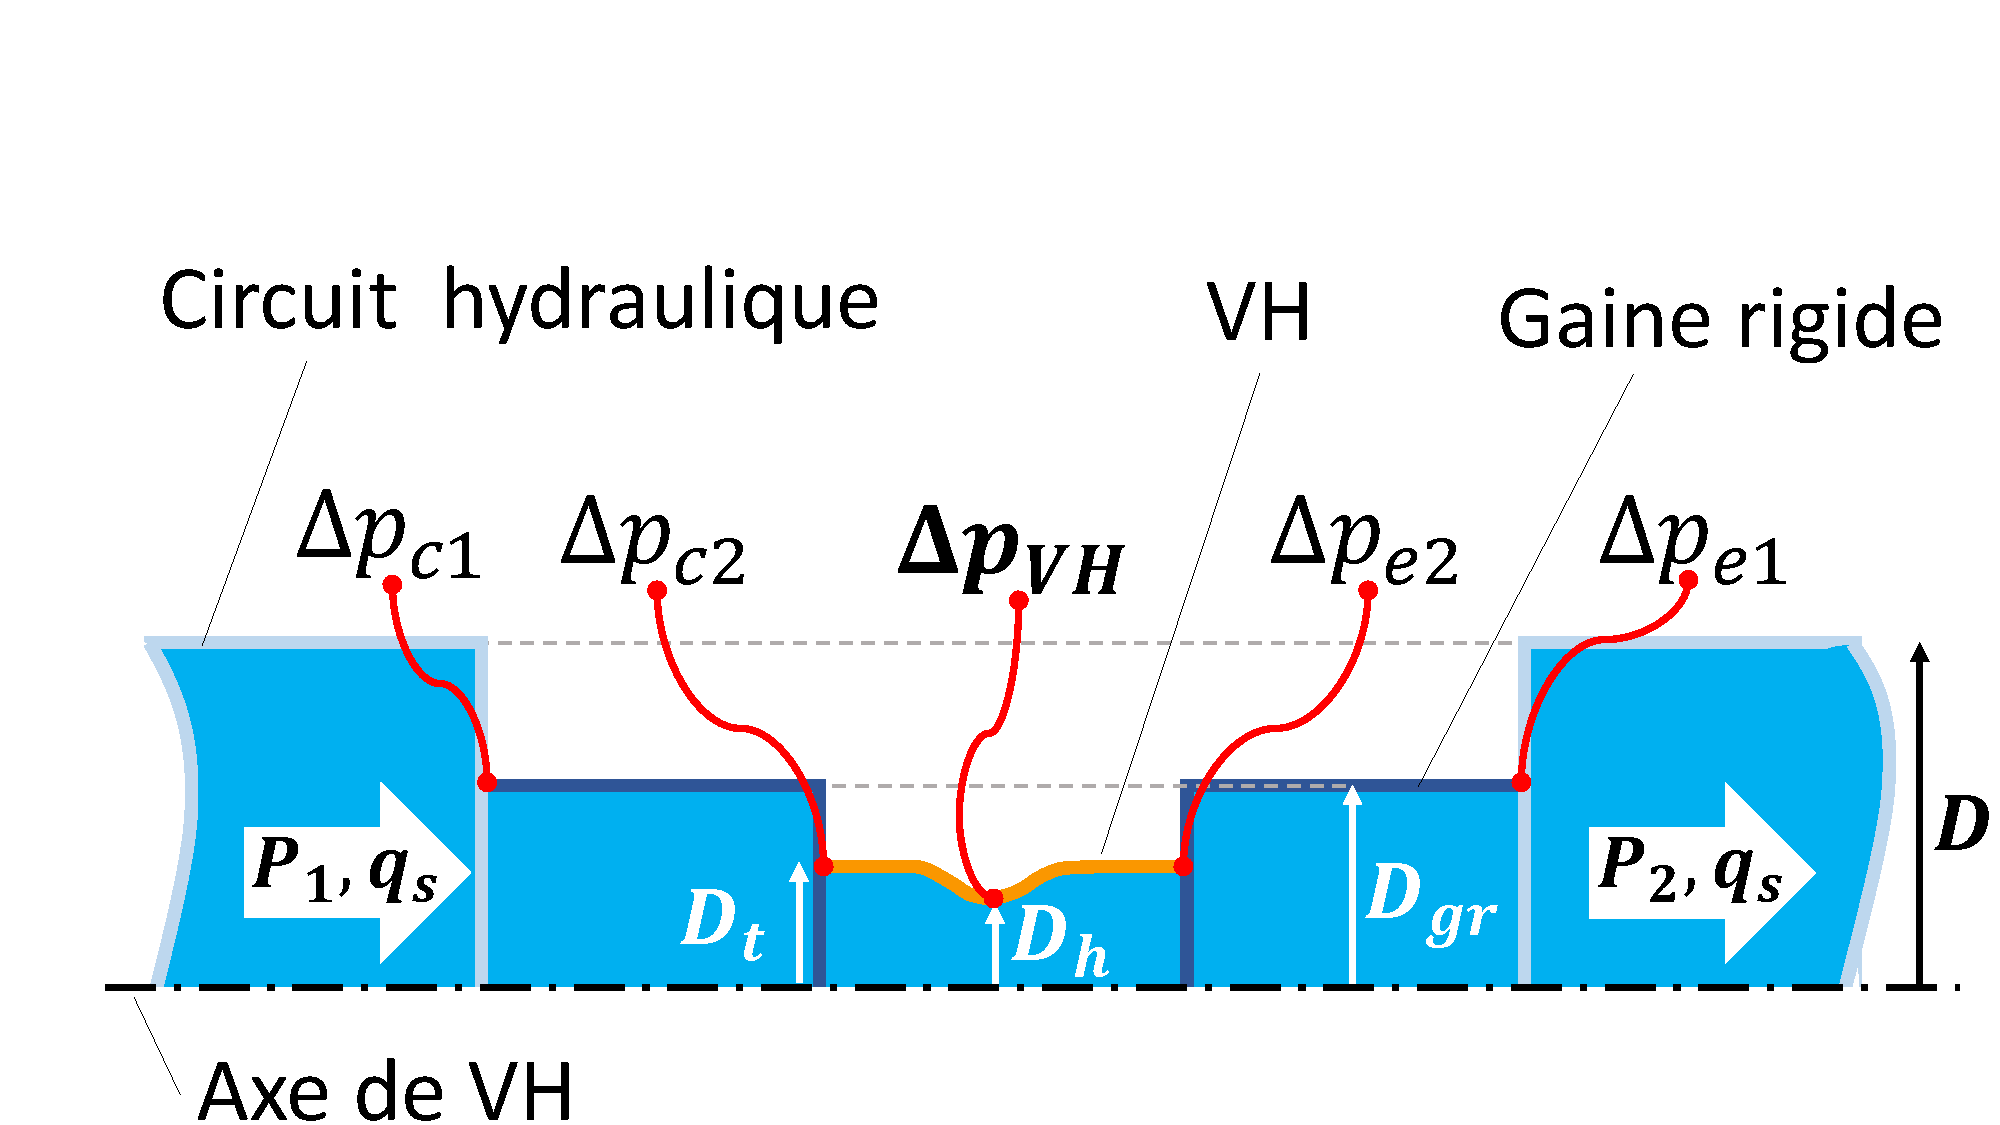
\includegraphics[trim={2cm 0cm 0cm 4cm},clip,width=0.6\textwidth]{../Chap4/Figure/fabrication_tube_experimental.pdf}
	\caption{Méthode de fabrication de la VH}
	\label{fig:fabrication_tube_experimental}
\end{center}	
\end{figure}    
%%%%%%%%%%%%%%%%%%%%%%%%%%%%%%%%%%%% 
    %/////////////////////////////////////////////	
	\subsection{Résultats et discussion}
	\label{subsec:4.4.2_Resultats et discussion}    
    %/////////////////////////////////////////////    		   
Nous avons réalisé 7 vidanges successives de la seringue en incrémentant $\theta$ de \ang{0} à \ang{60} pour chacune d'elles. Les capteurs de pression admettant une pression maximale de 25kPa pour les besoins de précision, il est difficile d'aller chercher des angles au-delà de \ang{60} sans risquer de saturer le capteur P1 qui mesure alors la pression la plus élevée. En effet, la perte de charge dans la VH devient trop importante, nécessitant une pression amont plus élevée pour que l'écoulement se fasse. Pour chaque vidange, réalisée manuellement, nous avons gardé un débit constant pour faciliter l'extraction de $Cf_{VH}$. Après avoir filtré les signaux mesurés, nous avons tracé sur la figure \ref{fig:resultats_essais_hydraulique_P1,P2,Qe_D1mm} les résultats de volume $\Delta V_{ser}$ de la seringue et des pressions $p_1$ et $p_2$ avec un code couleur pour chaque incrément d'angle. Une troncature temporelle des données a été réalisée autour du moment où le débit $q_{ser}$ traduisant la pente de $\Delta V_{ser}(t)$ est quasi-constant. Néanmoins, les fluctuations de pressions peuvent paraître élevées en amont de la VH. En effet, les PdC singulières sont importantes et proportionnelles au carré du débit. Ce-dernier n'étant pas tout à fait constant, sa faible variation induit des variations de pression importantes.
%%%%%%%%%%%%%%%%%%%%%%%%%%%%%%%%%%%%	
\begin{figure}[!htb]
\begin{center}
    \captionsetup{justification=centering} 
	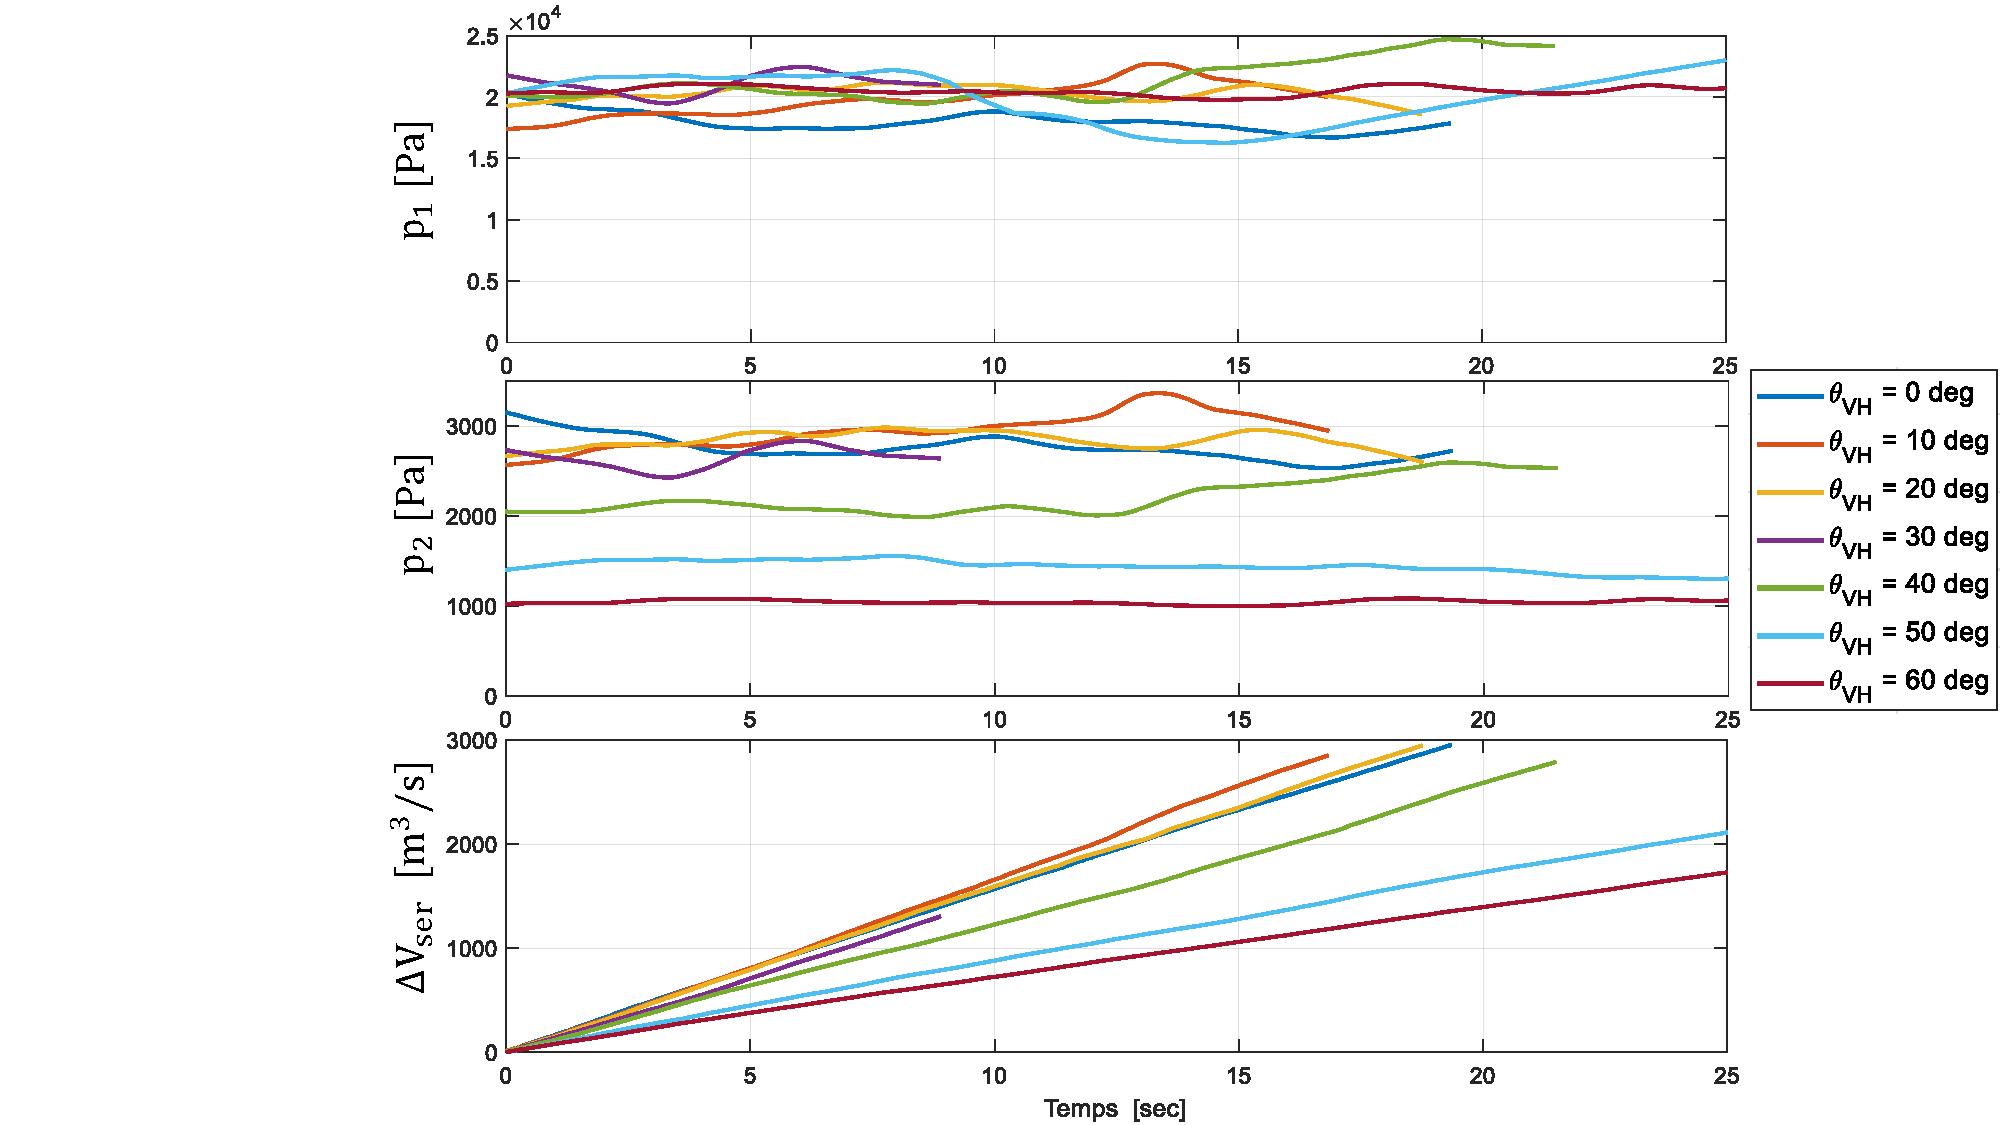
\includegraphics[trim={6cm 0cm 0cm 0cm},clip,width=\textwidth]{../Chap4/Figure/resultats_essais_hydraulique_P1,P2,Qe_D1mm.pdf}
	\caption{Essais de caractérisations hydrauliques de VH}
	\label{fig:resultats_essais_hydraulique_P1,P2,Qe_D1mm}
\end{center}	
\end{figure}    
%%%%%%%%%%%%%%%%%%%%%%%%%%%%%%%%%%%% 

Une approximation linéaire est faite sur les courbes de $\Delta V_{ser}(t)$, en supposant $q_{ser}$ constant. L'équation \ref{eq:Cf_VH_exp} permet alors de calculer $Cf_{VH}$ pour tous les incréments d'angle. Le résultat de $Cf_{VH}$ obtenu avec le jeu de données expérimentales pour les 7 angles testés est présenté sur la figure \ref{fig:resultats_essais_hydraulique_VH_D1mm}. L'étranglement hydraulique au niveau de la section flambée du tube T100p est remarquable sur l'évolution de $Cf_{VH}$. Les résultats des caractérisations statiques montrent que $K_t$ a une tendance décroissante pour le tube T100p à partir de $\theta\approx\ang{8}$ (fig. \ref{fig:(K_VH)_vs_theta_D1mm_plastifie}). $\theta_0$ sera donc préférablement fixé à une valeur supérieure à cet angle. Le rapport de fermeture expérimental $r_{cf,xp}$ est de 60 lorsqu'il est estimé pour un angle d'ouverture de \ang{20} et un angle de fermeture de \ang{60}. Le CdC hydraulique d'un VH stipule que le rapport minimal pour un fonctionnement correct est de $r_{cf}=10$ (fig. \ref{eq:Cf(x_m) evolution lineaire}). Ce tube assure donc, d'après le modèle théorique intégrant les données expérimentales, une bonne gestion directionnelle du fluide pour cycler le fonctionnement du système. 
%%%%%%%%%%%%%%%%%%%%%%%%%
\begin{figure}[!htbp]
	\begin{center}
		\captionsetup{justification=centering}
		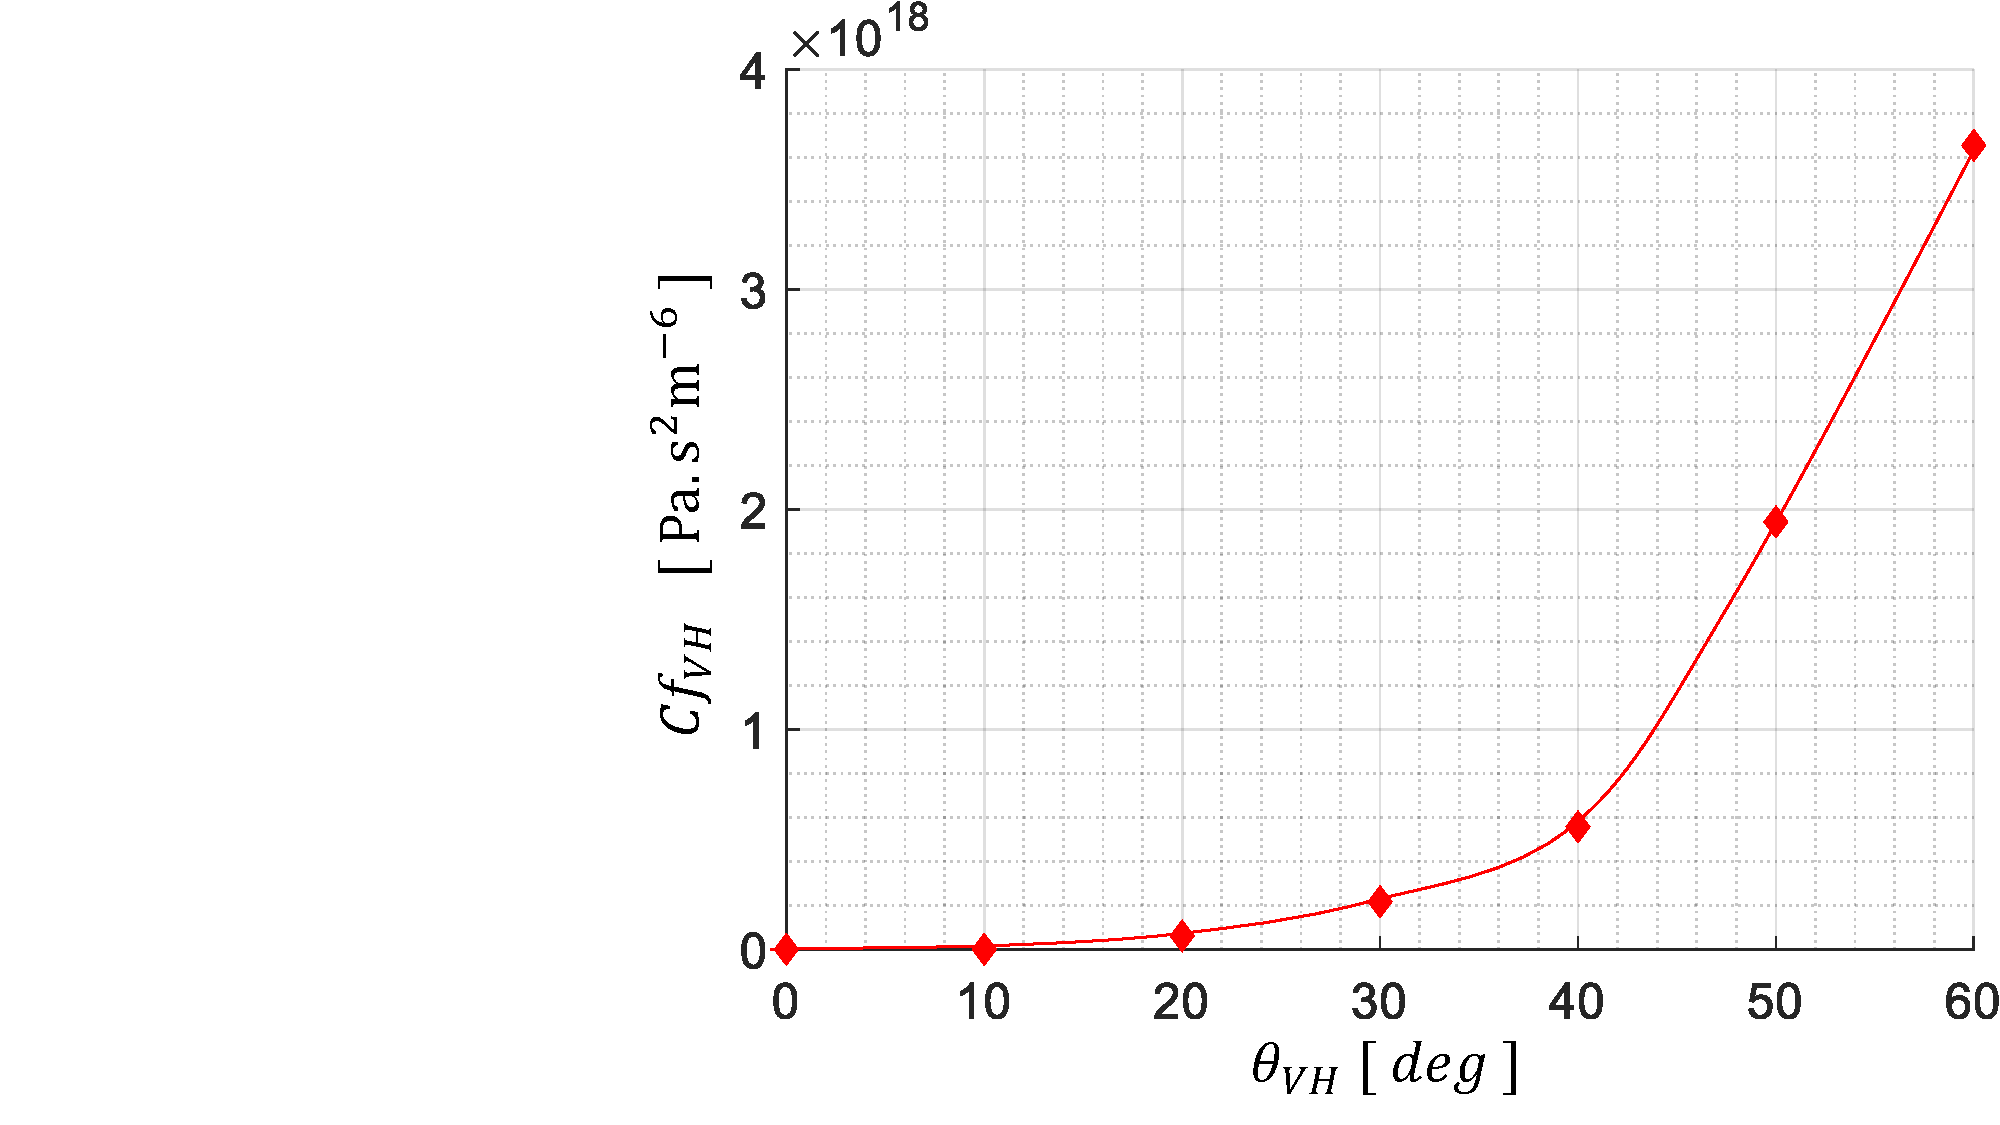
\includegraphics[trim={10cm 0cm 0cm 0cm},clip,width=0.6\textwidth]{../Chap4/Figure/resultats_essais_hydraulique_VH_D1mm.pdf}
		\caption{$Cf_{VH}$ calculé à partir des essais pour 7 incréments d'angles}
		\label{fig:resultats_essais_hydraulique_VH_D1mm}
	\end{center}
\end{figure}
%%%%%%%%%%%%%%%%

%/!\/!\/!\/!\/!\/!\/!\/!\/!\/!\/!\/!\/!\/!\/!\/!\/!\/!\/!\/!\/!\/!\/!\/!\ 		
\section{Caractérisation expérimentale du contact M-VH}
\label{sec:4.3_Caractérisations expérimentale du contact M-VH}
%/!\/!\/!\/!\/!\/!\/!\/!\/!\/!\/!\/!\/!\/!\/!\/!\/!\/!\/!\/!\/!\/!\/!\/!\ 	
    %///////////////////////////////////////////// 	
	\subsection{Présentation du banc de test}
	\label{subsec:4.3.1_Presentation du banc de test}
    %///////////////////////////////////////////// 	
Le banc de test développé a pour objectif d'étudier l'influence dynamique du contact M-VH. Les composants, ainsi que la configuration des essais, sont présentés sur la figure \ref{fig:presentation_BDT_lacher_tube}. On y retrouve les photos légendées au début et à la fin des essais dont le protocole est présenté dans la suite. La masse M se trouve en $-x_0$ avant actionnement et en $x_{0,vh}<x_0$ après. La flexion de la VH passe de $\theta_0$ avant actionnement à $\theta_f>\theta_0$ après.

Le banc est composé de l'OB implémentant le GPA et d'une VH constituée d'un tube T100p identique à celui utilisé lors des essais de caractérisation hydraulique (fig. \ref{fig:fabrication_tube_experimental}). Le point de contact M-VH à $x_m=0$ est réglé de façon à nous placer dans la configuration la plus proche possible de la prédiction théorique schématisée sur la figure \ref{eq:theta=f(x_m)}.
%%%%%%%%%%%%%%%%%%%%%%%%%%%%%%%%%
\begin{figure}[!htbp]
\begin{center}
	\begin{subfigure}[b]{0.49\textwidth}
    \captionsetup{justification=centering} 
	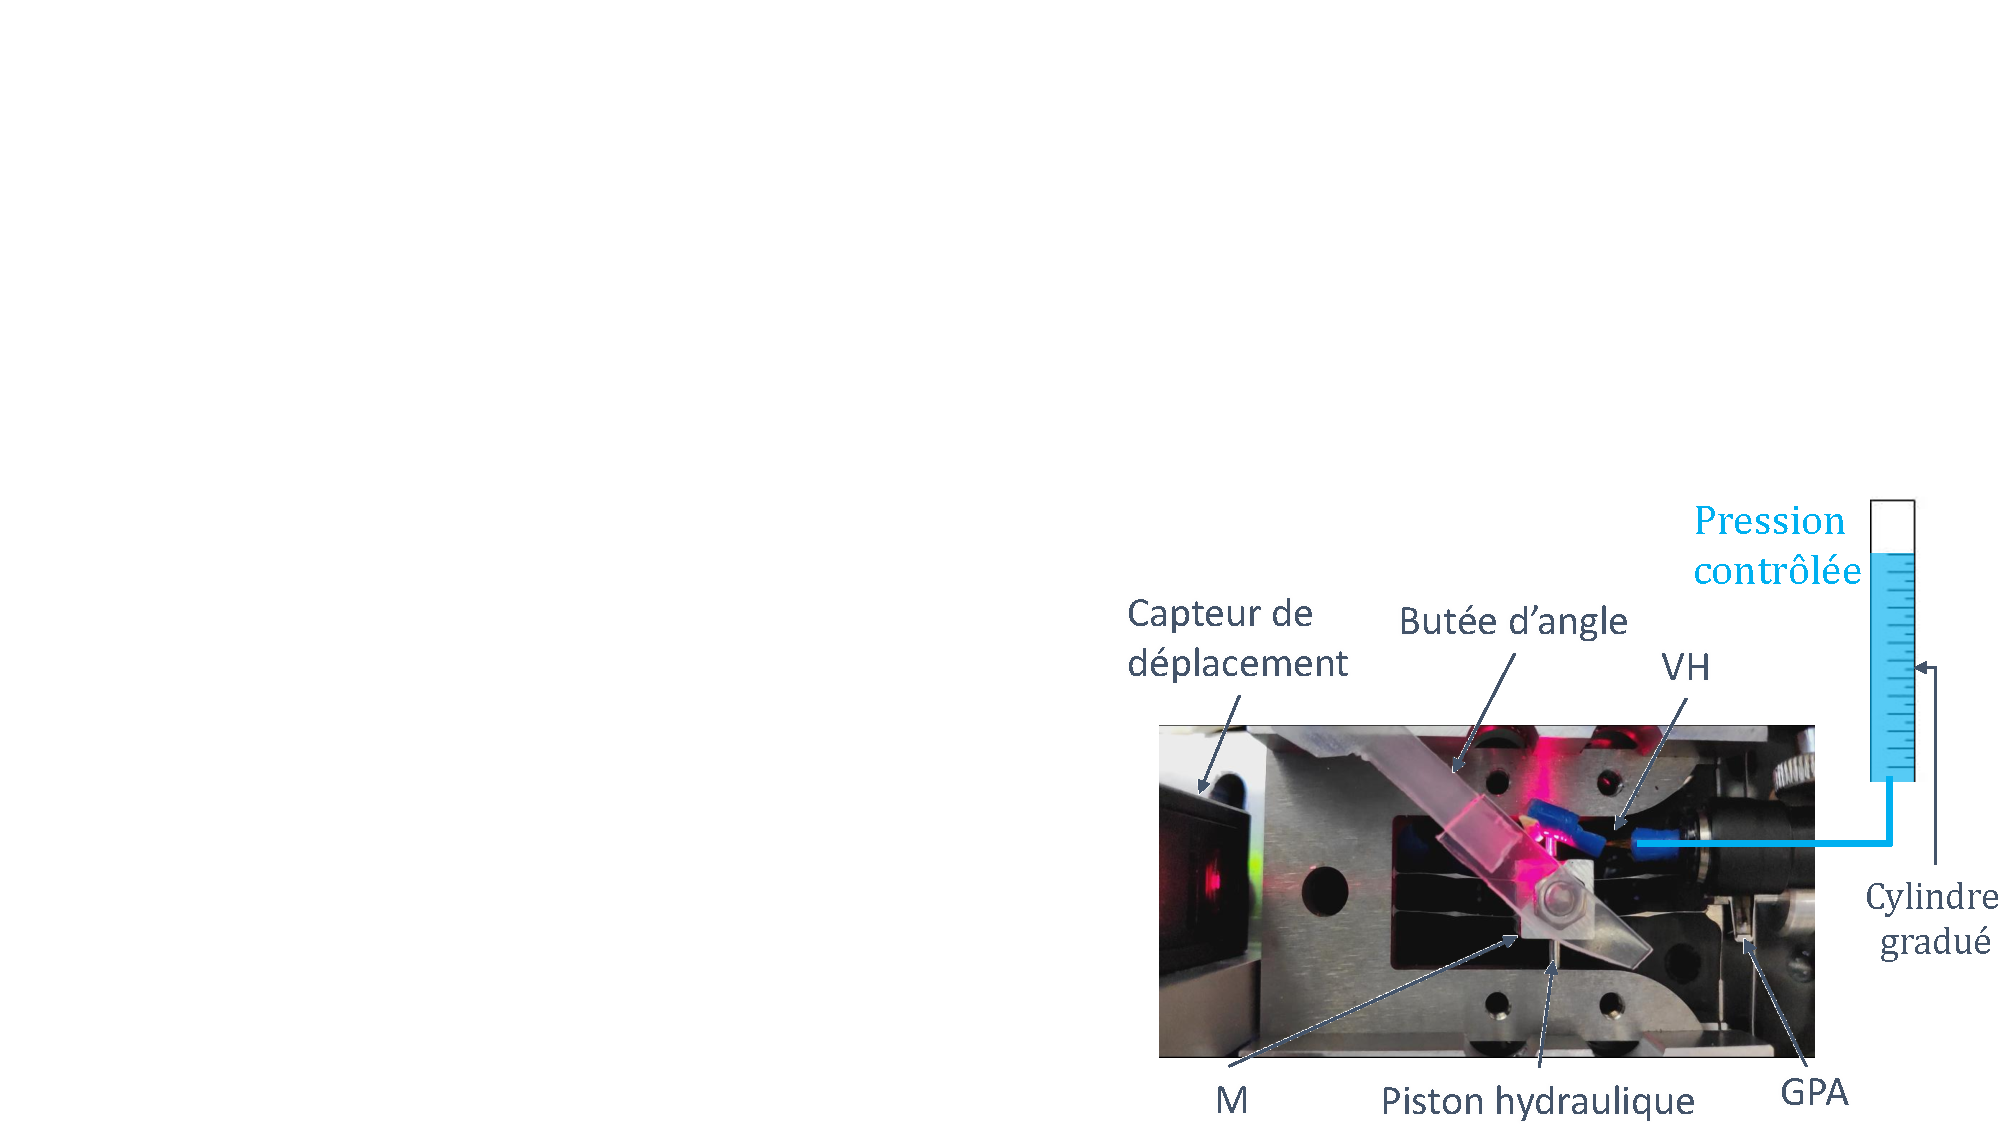
\includegraphics[trim={19cm 0cm 0cm 8cm},clip,width=\textwidth]{../Chap6/Figure/presentation_BDT_avant_actionnement.pdf}
	\caption{Avant lâcher : $x_m=-x_0$}
	\label{fig:presentation_BDT_lacher_avant_actionnement}
	\end{subfigure}
\hfillx
	\begin{subfigure}[b]{0.49\textwidth}
    \captionsetup{justification=centering} 
	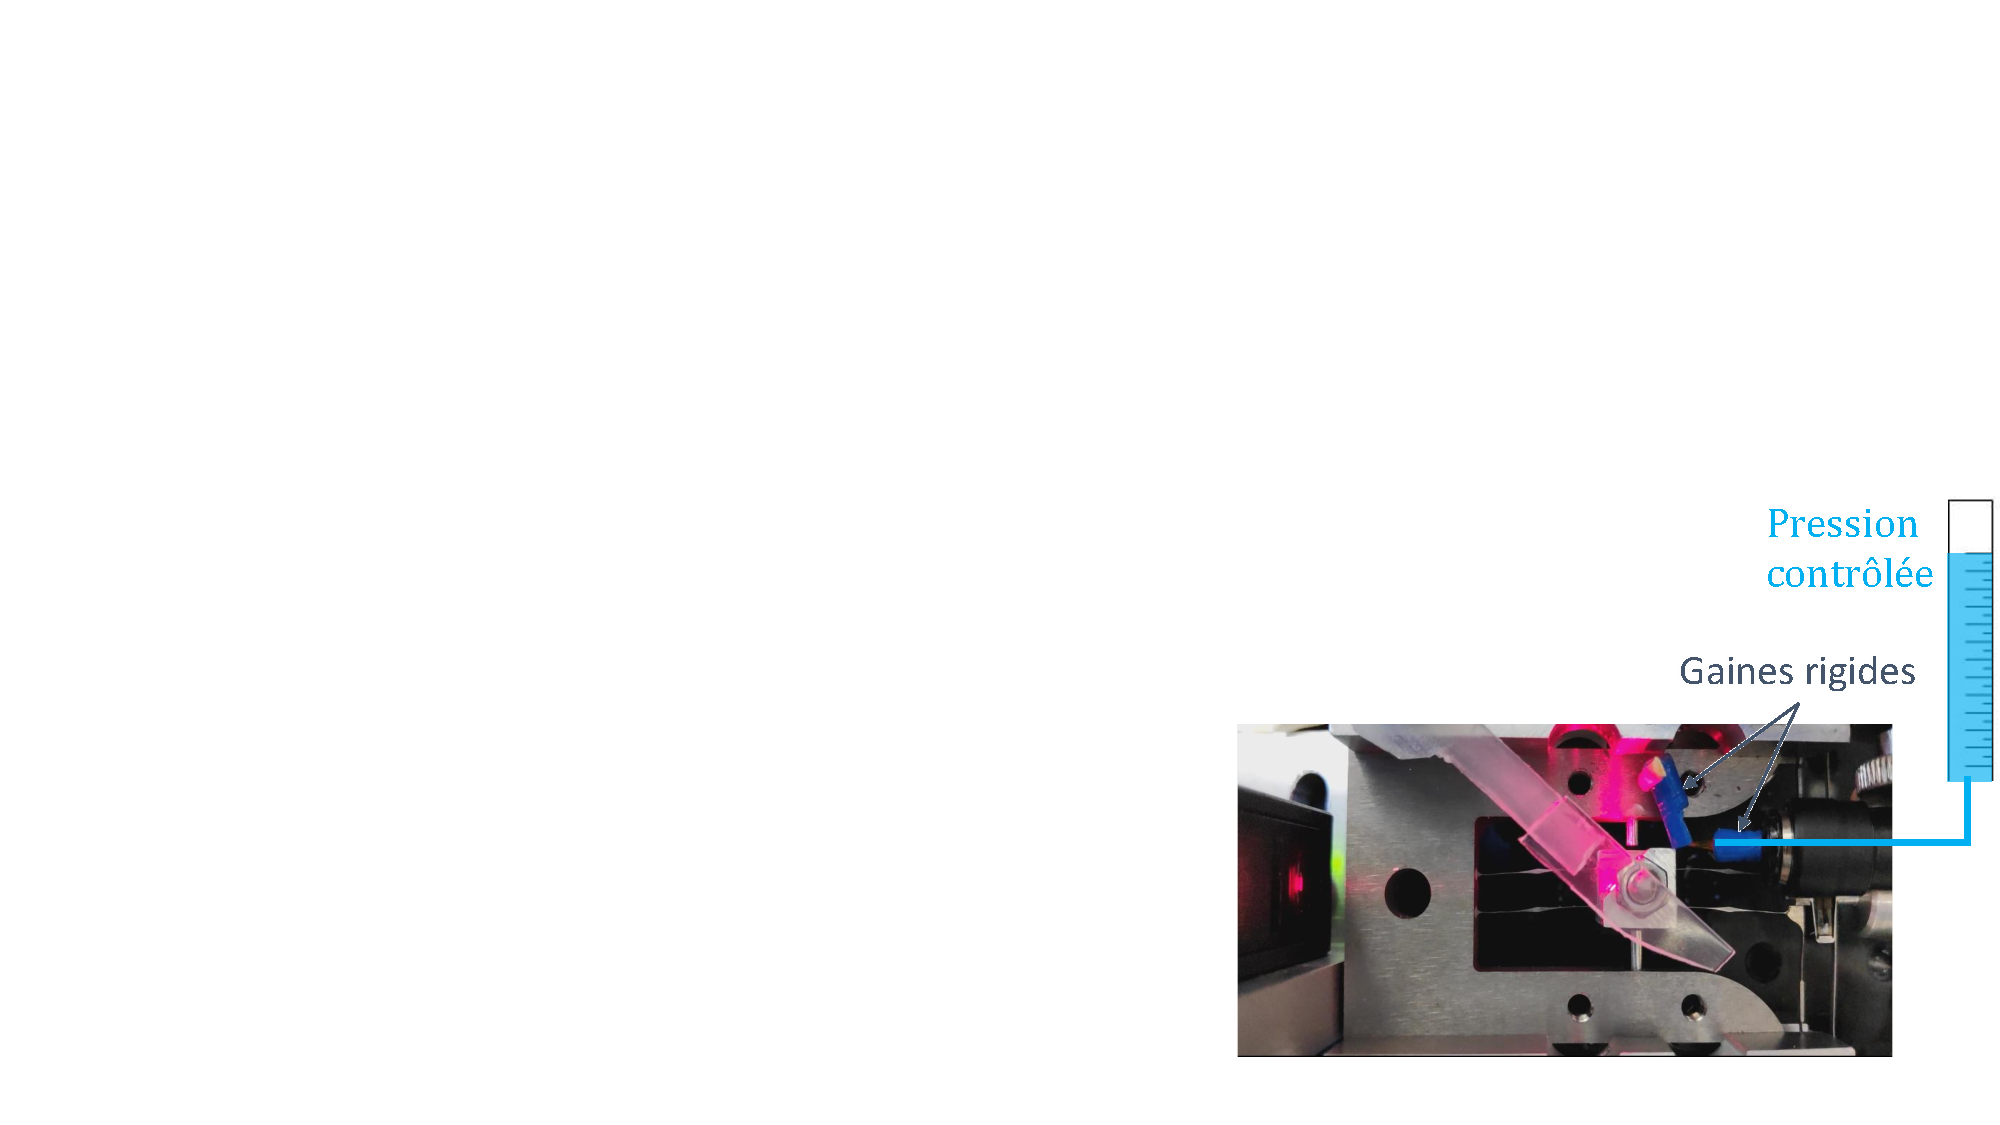
\includegraphics[trim={19cm 0cm 0cm 8cm},clip,width=\textwidth]{../Chap6/Figure/presentation_BDT_apres_actionnement.pdf}
	\caption{Après lâcher : $x_m=x_{0,vh}$}
	\label{fig:presentation_BDT_lacher_apres_actionnement}
	\end{subfigure}
	\caption{Présentation du banc de test de lâcher avec VH}
	\label{fig:presentation_BDT_lacher_tube}
\end{center}	
\end{figure} 
%%%%%%%%%%%%%%%%%%%%%%%%%%%%%%%%%
L'angle de départ $\theta_0$ de la VH est ajusté avec une butée d'angle mécanique qu'on peut voir sur les photos de la figure \ref{fig:presentation_BDT_lacher_tube}. La VH est scellée à l'extrémité mobile et connectée à un cylindre gradué à l'extrémité fixe. L'intérieur de la VH peut donc être pressurisé à sa pression de fonctionnement (10kPa) en gérant le niveau de fluide dans le cylindre. Le bras de levier de pliage a été ajusté manuellement autour du millimètre et sera plus précisément évalué par la suite.

La VH n'est présente que d'un seul côté, car les essais consistent à évaluer la dynamique vibratoire de la masse avec l'ajout de la VH, suivant la configuration voulue pour assurer son pliage. Le déroulement des tests consiste alors à pousser la masse depuis $x_m=-x_0$ jusqu'à $x_m=0$ et la laisser osciller avec la VH jusqu'à son arrêt en $x_m=x_{0,vh}$. Comme on a pu le faire précédemment, nous mesurons la position de M, ainsi que la tension $U_p$ aux bornes de la résistance de charge branchée sur les électrodes de sortie du GPA. Le niveau de flambement $x_0$ de l'OB a été réglé sur la même valeur que lors des tests de lâcher seul présentés dans le chapitre \ref{ch:3_Conception et fabrication du convertisseur electromecanique : OB + GPA}, soit $0.5$mm. Avant d'exploiter les résultats de mesures expérimentales, il est nécessaire d'ajuster le modèle théorique de l'évolution de $\theta$ en fonction de $x_m$. En effet, l'ajout d'une gaine rigide de diamètre supérieur à celui de la VH induit une cinématique différente de ce que prédit le modèle extrait de la figure \ref{eq:theta=f(x_m)}. La section qui suit présente alors l'évolution de la configuration de pliage.
    %///////////////////////////////////////////// 	
	\subsection{Évolution de la cinématique d'actionnement}
	\label{subsec:4.3.2_Evolution de la cinematique d'actionnement}
    %///////////////////////////////////////////// 	
Lorsque la masse et la valve entrent en contact, il est nécessaire que le déplacement de M induise une flexion sur la partie mobile de la VH. Or, le kapton constituant la VH est très souple devant l'acier constituant la masse. La VH risquerait de se déformer sous la contrainte de l'acier venant au contact. L'ajout de la gaine rigide (GR) autour de la VH assure alors un bon transfert des efforts mécanique exercés par M sur ce dernier. Cela permet d'assurer la fermeture de la section flambée de la VH. On remarque une première chose importante en prenant une image des positions respectives de M et VH au premier contact et après arrêt des oscillations. La figure \ref{fig:deplacement_zlat_xm=0} présente une image du premier contact et la figure \ref{fig:deplacement_zlat_xm=x0} illustre le contact lorsque M a fini d'osciller.
%%%%%%%%%%%%%%%%%%%%%%%%%%%%%%%%%
\begin{figure}[!htbp]
\begin{center}
	\begin{subfigure}[b]{0.49\textwidth}
    \captionsetup{justification=centering} 
	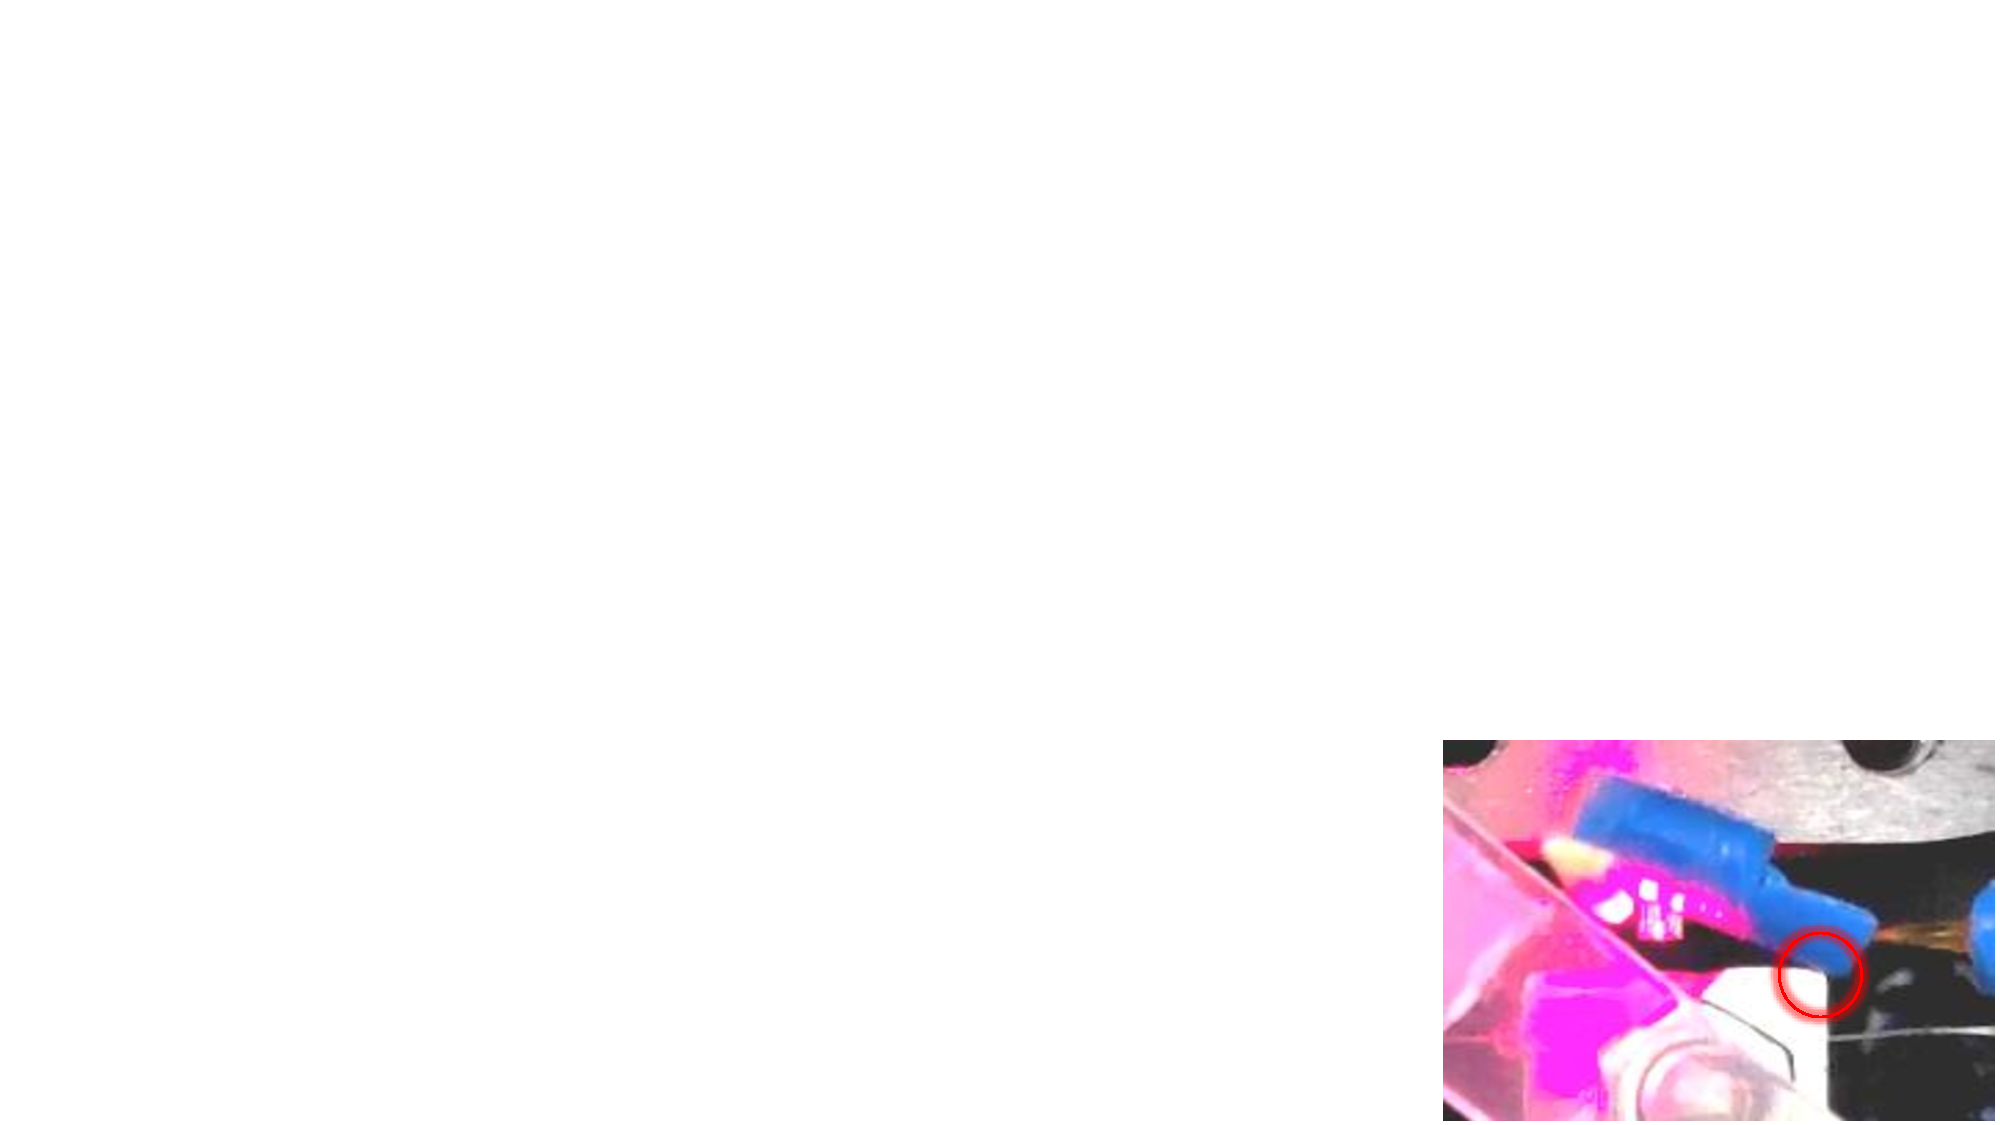
\includegraphics[trim={24.7cm 0cm 0cm 12.5cm},clip,width=\textwidth]{../Chap6/Figure/deplacement_zlat_xm=0.pdf}
	\caption{$x_0=0$}
	\label{fig:deplacement_zlat_xm=0}
	\end{subfigure}
\hfillx
	\begin{subfigure}[b]{0.49\textwidth}
    \captionsetup{justification=centering} 
	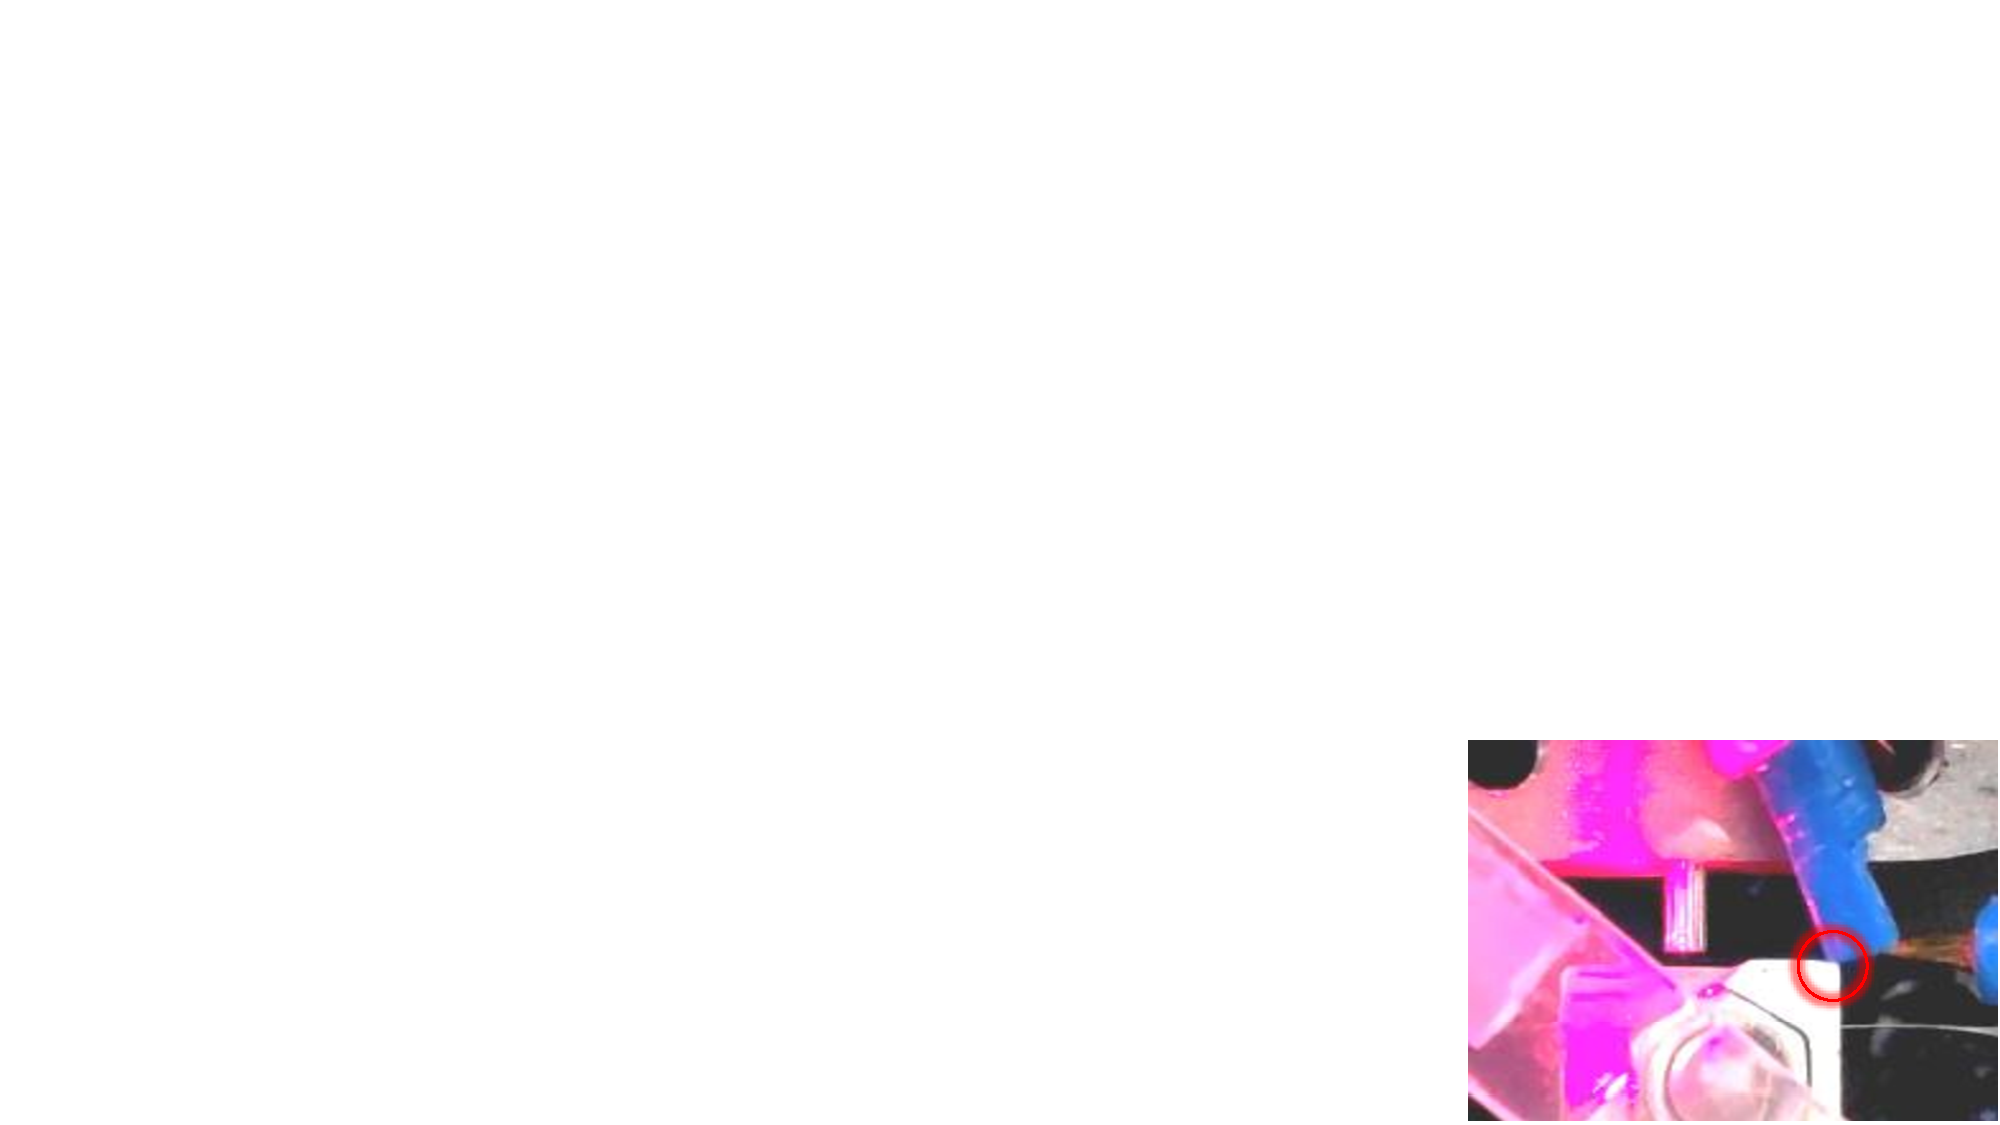
\includegraphics[trim={24.7cm 0cm 0cm 12.5cm},clip,width=\textwidth]{../Chap6/Figure/deplacement_zlat_xm=x0.pdf}
	\caption{$x_0=x_{0,vh}$}
	\label{fig:deplacement_zlat_xm=x0}
	\end{subfigure}
	\caption{Déplacement du point de contact M-VH}
	\label{fig:deplacement_zlat}
\end{center}	
\end{figure} 
%%%%%%%%%%%%%%%%%%%%%%%%%%%%%%%%%
%%%%%%%%%%%%%%%%%%%%%%%%%
\begin{figure}[!htbp]
	\begin{center}
		\begin{subfigure}[b]{0.49\textwidth}
			\captionsetup{justification=centering}
			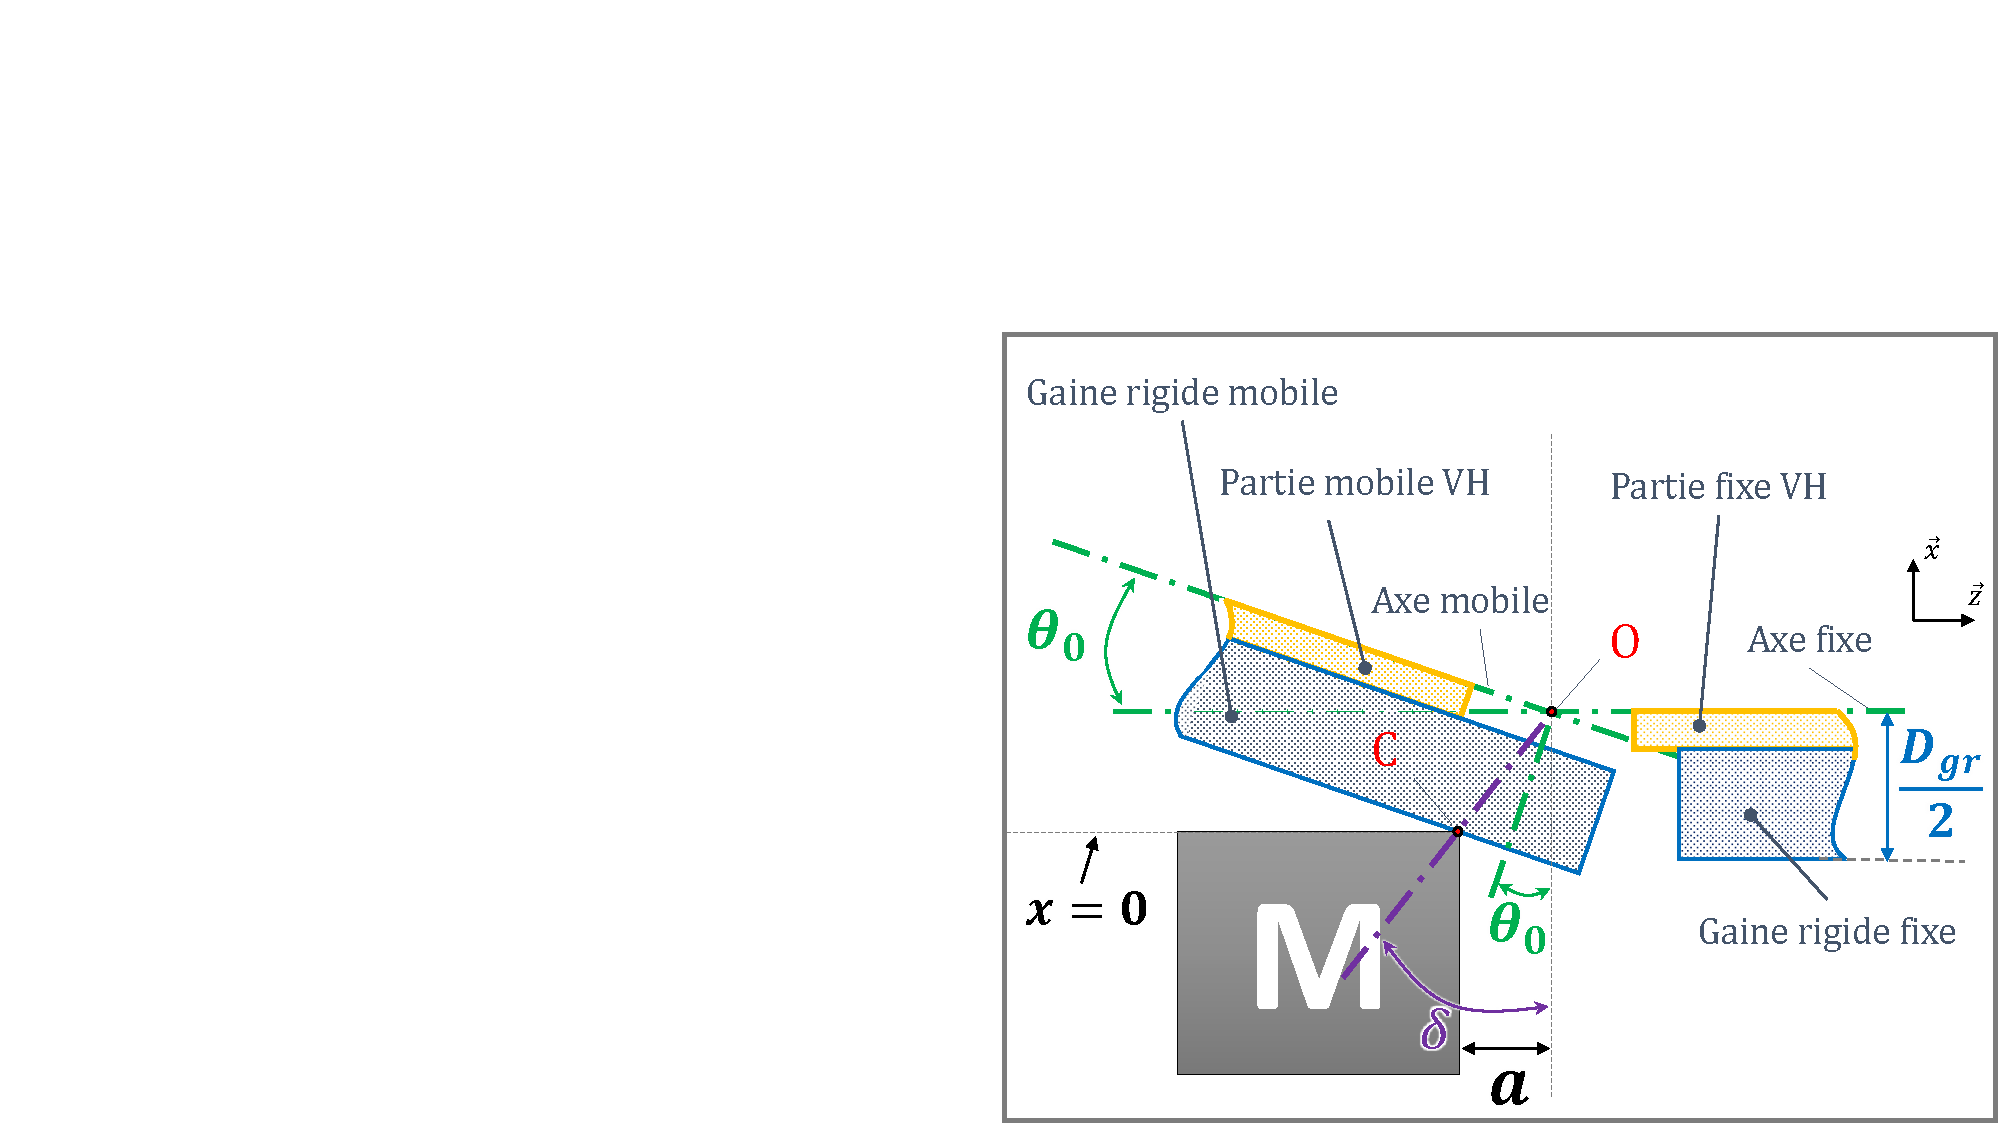
\includegraphics[trim={16.8cm 0cm 0cm 5.5cm},clip,width=\textwidth]{../Chap6/Figure/cinematique_pliage_VH_lacher_mini.pdf}
			\caption{Configuration du contact M-VH avant saut}
			\label{fig:cinematique_VH_avant-saut_mini}
		\end{subfigure}
		\hfillx
		\begin{subfigure}[b]{0.49\textwidth}
			\captionsetup{justification=centering}
			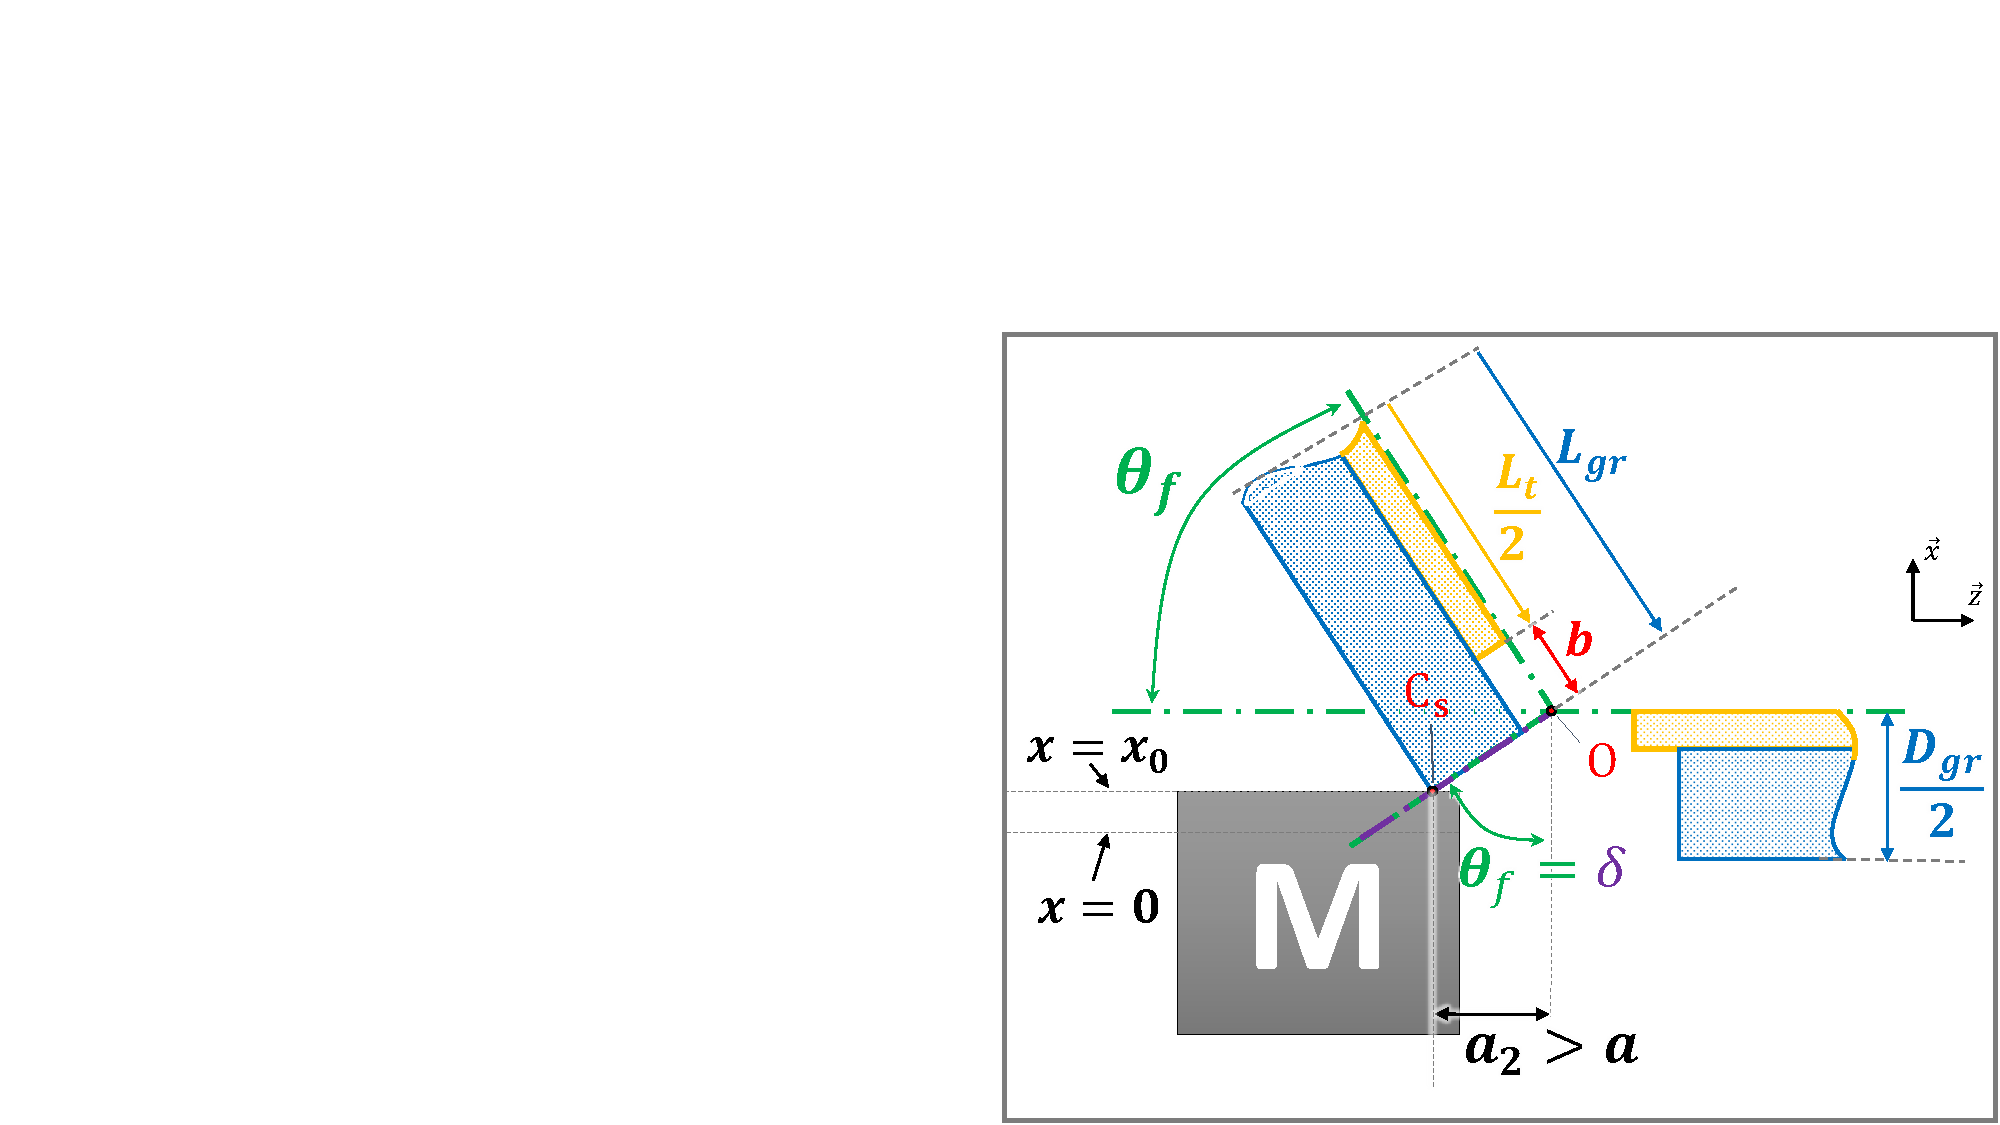
\includegraphics[trim={16.8cm 0cm 0cm 5.5cm},clip,width=\textwidth]{../Chap6/Figure/cinematique_pliage_VH_lacher_mini_saut.pdf}
			\caption{Configuration du contact M-VH après saut}
			\label{fig:cinematique_VH_après-saut_mini}
		\end{subfigure}
		\caption{Configuration du contact M-VH en fonction de la position de M}
		\label{fig:cinematique_VH_mini}
	\end{center}
\end{figure}
%%%%%%%%%%%%%%%%
Le point de contact M-VH, censé théoriquement rester l'arête supérieure droite de M, se retrouve en position finale sur sa face supérieure. Pour mieux comprendre ce phénomène on schématise les deux configurations, au premier contact lorsque $x_m=0$ et à la fin des oscillations lorsque $x_m=x_0$ sur la figure \ref{fig:cinematique_VH_avant-saut_mini}. On les qualifiera respectivement de contact \emph{latéral} et de contact \emph{supérieur}.

Ce phénomène apparaît seulement lorsque le diamètre $D_{gr}$ de la GR est supérieur à $2a$, avec $a$ étant le bras de levier nécessaire pour satisfaire $\Delta\theta$. En effet, à partir de l'angle limite $\theta(x_{ms})$ défini à l'équation \ref{eq:theta_max_av_saut}, il se produit le changement de configuration faisant intervenir le contact \emph{supérieur}. $x_{ms}$ représente alors l'abscisse limite de M pour cet angle.
\begin{equation}
	\theta(x_{ms})\ = \ \arctan\biggl(\dfrac{2a}{D_{gr}}\biggr)
	\label{eq:theta_max_av_saut}
\end{equation} 

Pour chacun des deux cas de contact, les lois d'évolution de $\theta$ avec la variation de $x_m$ ont été étudiées. Les détails des calculs sont présentés en annexe \ref{Ann:Annexe7_cinematique_M-VH}. 

Cette nouvelle cinématique de pliage est comparée avec celle qui a jusqu'ici été considérée dans le modèle (fig. \ref{fig:detail_flambement_MDOB}). Les résultats sont alors présentés et discutés dans la section qui suit. 
%///////////////////////////////////////////// 		
\subsection{Influence de la gaine rigide sur l'évolution de $\theta$}
\label{subsec:4.3.3_Influence de la GR sur l evolution de theta}
%/////////////////////////////////////////////
Cette section présente les résultats de l'étude comparative de la cinématique de pliage des VH pour deux cas de figure :
\begin{itemize}[label=$\bullet$]
	\item Le système OBVH où le tube kapton composant la VH ne possède pas de gaine rigide (GR) : ce cas de figure est référencé par le système OBVH$_{sg}$.
	\item Le système OBVH où le tube kapton composant la VH possède une GR : ce cas de figure est référencé par le système OBVH$_{ag}$. Ce cas de figure se décompose lui-même en 3 configurations qui dépendent de $b$ défini à l'équation \ref{eq:b_definition}.
	      \begin{itemize}[label=$\circ$]
		      \item	Configuration 1 : $b > 0$
      		  \item Configuration 2 : $b = 0$
			  \item Configuration 3 : $b < 0$
	      \end{itemize}
	Sachant que $b$ représente la différence entre les longueurs respectives $\frac{L_t}{2}$ de la partie mobile en kapton et $L_{gr}$ de la GR mobile (fig. \ref{fig:cinematique_VH_mini})
\end{itemize}
\begin{equation}
	b = \dfrac{L_t}{2} - L_{gr}
	\label{eq:b_definition}
\end{equation}
En prenant compte le diamètre $D_{gr}$ de la GR, l'évolution du contact \emph{latéral} au \emph{supérieur} a tendance à rigidifier l'articulation en $O$ de la VH. En effet, le dimensionnement de $a$ est pensé de manière à plier la VH sur la plage d'angle $\Delta\theta$ lorsque $x_m$ varie entre 0 et $x0_{vh}$. Cependant, on sait que lors des oscillations, $x_m$ devient plus grand que $x0_{vh}$ et, par conséquent, $\theta$ varie au-delà de la borne supérieure de $\Delta\theta$. Si $2a<D_{gr}$, la VH finit par atteindre l'angle de basculement $\theta_(x_{ms})$ défini à l'équation \ref{eq:theta_max_av_saut} et il s'ensuit l'apparition de la configuration de contact \emph{supérieur}, changeant ainsi la dynamique de pliage.

Pour de très faibles variations de $x_m$, il se produit une importante variation de $\theta$ (fig. \ref{fig:theta_saut}) lorsque celui-ci approche de la limite de changement de configuration. Ce phénomène est intéressant du point de vue de l'étranglement hydraulique. Il peut être quantifié en comparant les cinématiques de pliage avec et sans GR. Pour ce faire, nous allons nous servir du modèle de l'OB recalé suite aux essais expérimentaux du chapitre \ref{ch:3_Conception et fabrication du convertisseur electromecanique : OB + GPA}, ainsi que des données expérimentales hydrauliques et statiques issues des essais sur le tube T100p.
%%%%%%%%%%%%%%%%%%%%%%%%%
\begin{figure}[!htb]
\begin{center}
	\begin{subfigure}[b]{0.49\textwidth}
    	\captionsetup{justification=centering}
		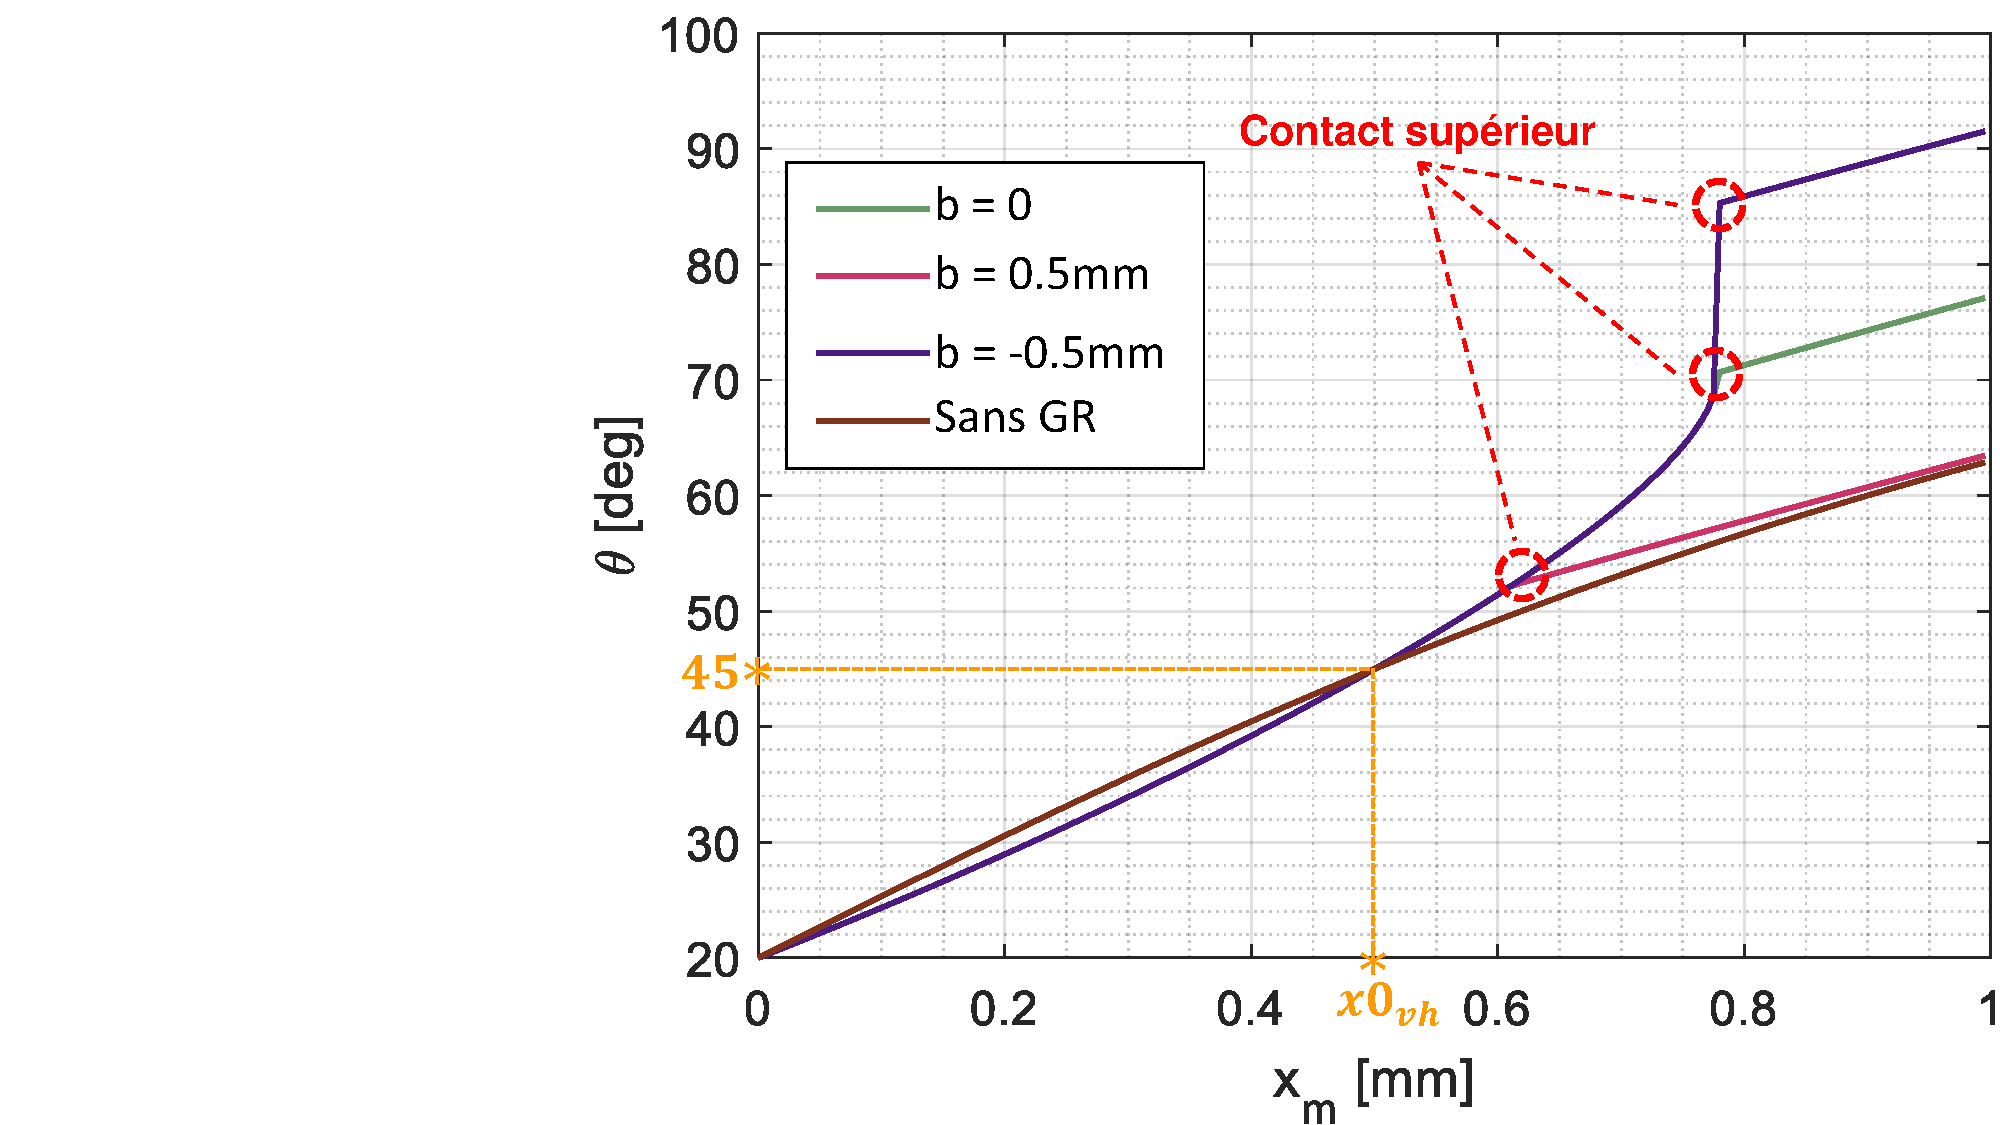
\includegraphics[trim={10cm 0cm 0cm 0cm},clip,width=.96\textwidth]{../Chap6/Figure/theta_vs_xm_avec_et_sans_gaine_tot.pdf}
		\caption{Évolution de $\theta$ en fonction de $x_m$}
		\label{fig:theta_vs_xm_avec_et_sans_gaine_tot}
	\end{subfigure}
\hfillx
	\begin{subfigure}[b]{0.49\textwidth}
    	\captionsetup{justification=centering}
		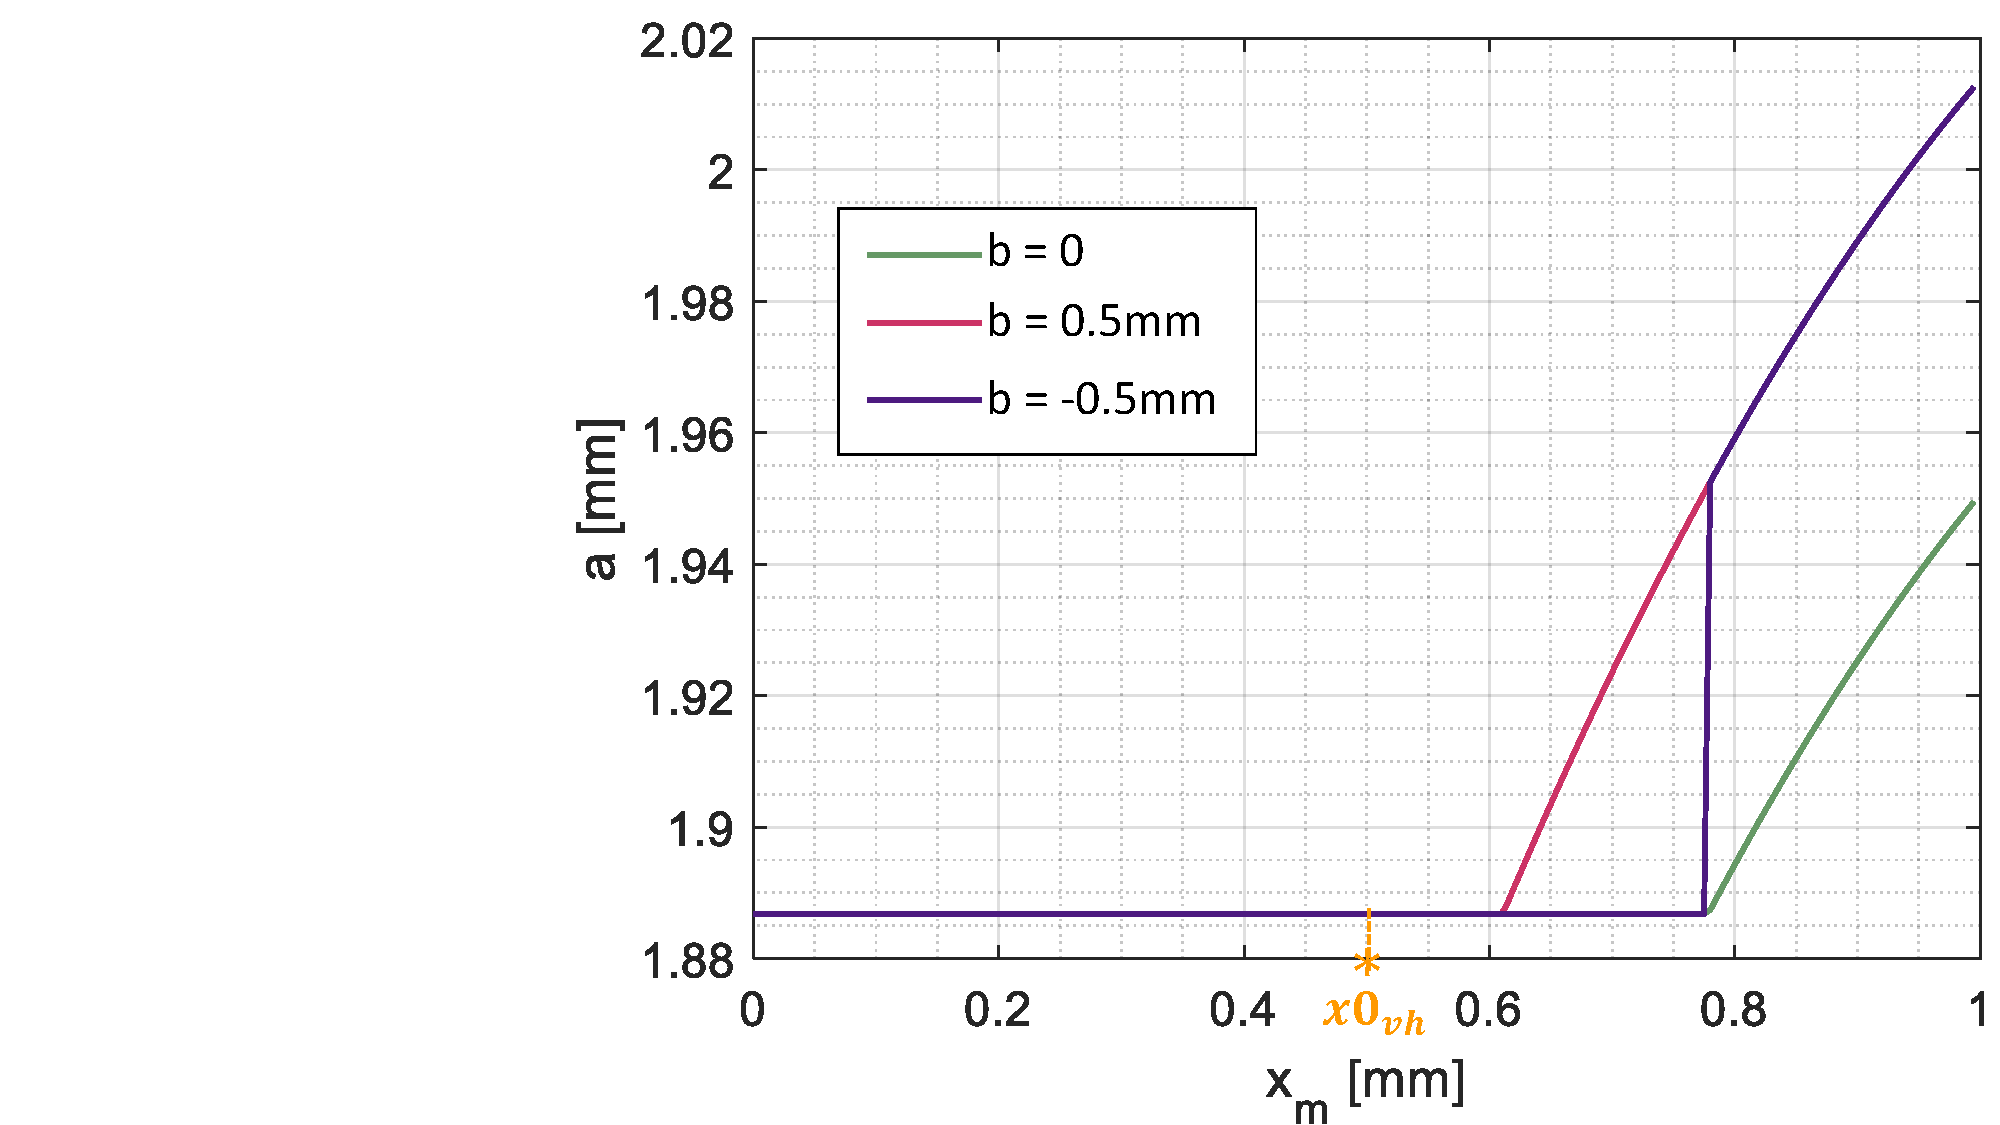
\includegraphics[trim={9.5cm 0cm 0cm 0cm},clip,width=.99\textwidth]{../Chap6/Figure/a_vs_xm_avec_et_sans_gaine_tot.pdf}
		\caption{Évolution de $a$ en fonction de $x_m$}
		\label{fig:a_vs_xm_avec_et_sans_gaine_tot}  
	\end{subfigure}
	\caption{Comparaison de la configuration cinématique M-VH en fonction de la GR pour différentes valeurs de $b$}
	\label{fig:(theta&a)_vs_xm_avec_et_sans_gaine_tot}
\end{center}	
\end{figure} 
%%%%%%%%%%%%%%%%   

Les simulations avec les deux configurations se placent dans les conditions initiales identiques aux tests de lâchers expérimentaux libres réalisés dans le chapitre \ref{ch:3_Conception et fabrication du convertisseur electromecanique : OB + GPA}. La position d'équilibre finale $x_{0,vh}$ et la plage de variation d'angle $\Delta\theta$ sont imposés identiques pour les deux systèmes OBVH$_{sg}$ et OBVH$_{ag}$, respectivement avec et sans GR. Les équations \{\ref{eq:x_0f} -  \ref{eq:S_ap}\} décrivent alors le comportement de l'OBVH$_{ag}$. De plus, l'équation \ref{eq:theta=f(x_m)}, établie précédemment dans le cas où le diamètre de la GR et celui de la VH sont égaux, décrit le comportement de l'OBVH$_{sg}$. Le tableau \ref{tab:comparaison_AG-SG} montre alors la comparaison entre les deux modèles sur certains paramètres critiques pour le fonctionnement du système. De plus, la figure \ref{fig:(theta&a)_vs_xm_avec_et_sans_gaine_tot} met en évidence la différence de l'évolution de $\theta$ et $a$ en fonction de $x_m$ pour les deux modèles, en considérant aussi différentes valeurs pour $b$.
	%%%%%%%%%%%%%%%%%%%%%%%%%%%%%%%%%%%%	
\begin{table}[!htbp]
	\centering
		\begin{tabular}[t]{|c||c|c|}
\hline
\textbf{Paramètre} & \textbf{Valeur OBVH$_{sg}$ théorique} & \textbf{Valeur OBVH$_{ag}$ théorique} \\
\hline \hline
$D_{gr}$ [mm] 						& \multicolumn{2}{|c|}{0.5}  \\ \hline
$\Delta\theta$ [deg] 			& \multicolumn{2}{|c|}{[\ang{20};\ang{45}]} \\
\hline
$K_{T100p}(\theta_f)$ [Nmm/rad] & \multicolumn{2}{|c|}{0.16} \\ \hline
$x_{0,vh}$ [mm] 				& \multicolumn{2}{|c|}{0.5}  \\ \hline
$x_{0}$  [mm]  					& 6.56 		&	5.94		 \\ \hline
$x_{0}\ /\ x_{0,vh}$ [\%] 		& 13.1		&	11.9		 \\ \hline
$a$		   [mm]         		& 1.07 		&	1.88 		 \\ \hline
$Ep_{bar}(OBVH)$ [$\micro$J]    & 8.4 		& 	10.4		 \\ \hline
$Ep_{bar}(OBVH)\ /\ Ep_{bar}(OB)$ [\%]  & 25    &    46		     \\ \hline
		\end{tabular}
        \caption{Valeur des paramètres de l'OBVH, à l'équilibre statique avec le tube T100p pour $\Delta\theta=[\ang{20};\ang{45}]$}
        \label{tab:comparaison_AG-SG}
\end{table}        
%%%%%%%%%%%%%%%%%%%%%%%%%%%%%%%%%%%%	

À titre de comparaison, b peut prendre trois valeurs que sont $b=-0.5mm$, $b=0mm$, et $b=0.5mm$ sur la figure \ref{fig:(theta&a)_vs_xm_avec_et_sans_gaine_tot}. La tendance de l'évolution de $\theta$ semble indépendante de l'utilisation de la GR lorsque $x_m\in[0;x_{0,vh}]$. Pour des valeurs supérieures à $x_{0,vh}$, la VH$_{ag}$ a cependant tendance à fléchir plus fort que la VH$_{sg}$, notamment dans les cas de figure où $b\leq 0$. La position de M, menant au basculement des configurations de pliage des VH$_{ag}$, du contact \emph{latéral} au \emph{supérieur}, est mise en évidence par le changement de l'allure des courbes respectives selon $b$. Cette position reste inchangée lorsque $b \leq 0$, mais apparaît cependant pour des angles plus faibles lorsque $b > 0$.

L'évolution de $\theta$ durant la configuration de contact \emph{supérieur} semble plus lente que pour une architecture sans GR. La fabrication de VH telles que $b>0$ a donc tendance à réduire leur variation de $\theta(x_m)$. Augmenter $b$ risque alors de mener à un étranglement hydraulique trop lent pour la VH$_{ag}$. Néanmoins, un compromis sur $b$ peut être réalisé en s'assurant que $x_{ms}>x_{0,vh}$, ce qui assurerait le respect du CdC hydraulique de la VH$_{ag}$.

Sur le plan énergétique, il semblerait d'après les valeurs calculées du tableau \ref{tab:comparaison_AG-SG}, que pour satisfaire un CdC hydraulique identique de la VH, $a$ est nettement plus faible dans une architecture comprenant une GR. L'OBVH$_{ag}$ admet une barrière énergétique plus importante que  L'OBVH$_{sg}$ pour une hauteur de flambement similaire. L'OB nécessite un niveau de flambement plus important dans l'architecture sans GR et, par conséquent, le niveau de flambement maximal $x_{0,max}$(tab. \ref{tab:x0max}) est plus facilement atteignable que dans l'architecture avec GR. Cette-dernière semble donc théoriquement apporter une plus-value conséquente au fonctionnement du système. En effet, le CdC hydraulique de la VH est satisfait et la résistance structurelle de l'OB est mieux préservée que sans la GR. L'influence énergétique de la VH est donc diminuée sur l'OB grâce à la nouvelle cinématique de pliage apportée par la GR.

La VH devrait donc être préférablement fabriquée avec une GR afin de réduire son influence énergétique sur l'OB et d'augmenter son étranglement hydraulique. Le réglage de $a$ est directement dépendant de CdC hydraulique $\Delta\theta$. Si $2a<D_{gr}$, le changement de configuration de contact risque d'avoir lieu (passage du \emph{latéral} au \emph{supérieur}). Une conception impliquant un congé sur les arêtes de M en contact avec la VH permettrait d'éviter ce changement brusque qui a tendance à rigidifier la VH. Une nouvelle modélisation cinématique serait alors nécessaire avec la prise en compte du rayon des congés réalisés.

D'autre part, la GR mobile devrait être fabriquée de façon à ce que le rapport entre sa longueur $L_{gr}$ et la longueur $L_t$ du tube kapton soit le suivant :
\begin{equation}
	\dfrac{L_t}{2} \leq L_{gr}
\end{equation}
Cela serait intéressant pour tirer profit de la forte variation de $\theta$ pour une faible variation de $x_m$ (fig. \ref{fig:theta_vs_xm_avec_et_sans_gaine_tot}).
%/!\/!\/!\/!\/!\/!\/!\/!\/!\/!\/!\/!\/!\/!\/!\/!\/!\/!\/!\/!\/!\/!\/!\/!\%
	\section{Conclusions de l'étude expérimentale des VH}
	\label{sec:4.5_Conclusions de l etude experimentale des VH}
%/!\/!\/!\/!\/!\/!\/!\/!\/!\/!\/!\/!\/!\/!\/!\/!\/!\/!\/!\/!\/!\/!\/!\/!\%
On a présenté sur la figure \ref{fig:(K_VH)_max(a)_et_Deltatheta_pour_bistabilite} la raideur $K_{VH}$ admissible sur l'OB fabriqué et présenté dans le chapitre précédent. Un banc de test spécifique a alors été développé pour la caractérisation statique de quatre tubes en kapton (fig. \ref{fig:BDT_statique_VH} et \ref{fig:essais_statique_total}) : T50, T100, T200 et T300 dont les dimensions sont présentées dans le tableau \ref{tab:dim_tube_statique}. Il en a résulté que le tube T50 est le seul dont la raideur est admissible sur l'OB monobloc. Une astuce technique a été de plastifier localement, à la section flambée, les 4 tubes précédemment testés, afin d'assouplir localement l'articulation au point de rotation. Les essais sur les tubes plastifiés ont révélé que le tube T100 plastifié (T100p) devient alors un choix envisageable, en plus du tube T50p. Pour faciliter la manipulation et l'installation de la VH, on choisit de continuer l'étude avec le tube T100p dont la raideur, en fonction de son angle de flexion, est présentée sur la figure \ref{fig:(K_VH)_vs_theta_D1mm_plastifie}.

Le dimensionnement préliminaire des VH, résultant des simulations présentés à la section \ref{subsec:2.5.3:Simulation et resultats}, ont montré qu'un rapport de fermeture $(r_{Cf})_{min}=10$ est nécessaire entre les deux valves ouvertes et fermées afin d'assurer la bonne commutation hydraulique.

Une VH a alors été fabriquée à base d'un échantillon de tube T100p identique à celui précédemment caractérisé sur le banc statique (fig. \ref{fig:fabrication_tube_experimental}). Un banc spécifique a été développé pour la caractérisation hydraulique des VH à base de tubes flexibles (fig. \ref{fig:BDT_hydraulique_VH} et \ref{fig:essais_hydraulique_VH}). Le comportement hydraulique du tube T100p a montré qu'un rapport d'étranglement $r_{Cf})=60$ est atteignable sur la plage d'angle de flexion $\Delta\theta =[\ang{20};\ang{60}]$ (fig. \ref{fig:resultats_essais_hydraulique_VH_D1mm}). Comme le comportement statique,le comportement hydraulique du tube T100p s'est expérimentalement révélé prometteur pour remplir le rôle de VH dans le système de récupération d'énergie.
	
Il a été constaté que l'ajout d'une GR, de diamètre supérieur à celui du tube constituant la valve, change la configuration de pliage de cette dernière. L'influence positive de la GR du point de vue du CdC de la VH a été mis en évidence et les systèmes d'équations définissant la nouvelle cinématique de mouvement ont été établis en annexe \ref{Ann:Annexe7_cinematique_M-VH}. Des préconisations de conceptions ont été données afin d'optimiser le contact M-VH. Les corrélations modèle-essais avec les nouvelles configurations de pliage seront présentées dans le chapitre \ref{ch:6_Comportement du systeme de recuperation d’energie intra-auriculaire avec les composants caracterises experimentalement}.
	
Les méthodes de fabrication utilisées pour mettre en \oe{}uvre la VH à base d'échantillon de tube T100p est discutable sur plusieurs points. Premièrement, la plastification locale est réalisée manuellement, ce qui rend sa répétabilité faible. De plus, il n'y a pas eu de caractérisations du vieillissement d'un tube ayant subi ces contraintes de plastification. Ces deux facteurs majeurs rendent un dimensionnement difficile, notamment sur le comportement statique de la VH.

Le chapitre suivant propose alors une méthode de dimensionnement théorique pour une VH afin d'avoir un modèle prédictif pouvant s'adapter aux changements du CdC du système. La pertinence du modèle sera discutée et les résultats seront mis en parallèle avec les données expérimentales.


% LIGNE 93	 	 
%	 	 L'énergie $(Ep_{OB})_{max}$ nécessaire pour amener la masse M de  l'OB depuis la position $x_m = x_{0,max}$ à la position $x_m=0$ peut alors être donnée par l'équation \ref{eq:(Ep_VH)_max}
%\begin{equation}
%	(Ep_{OB})_{max} = \dfrac{K{x_{0,max}}^4}{2L^2}
%\label{eq:(Ep_OB)_max}
%\end{equation} 	
%Si on suppose que la VH est un ressort rotatif linéaire, l'énergie élastique emmagasinée dans ce dernier lorsque $x_m$ varie entre $0$ et $x_{0,max}$ peut être exprimée par l'équation \ref{eq:(Ep_VH)_max}
%\begin{equation}
%	(Ep_{VH})_{max} =\dfrac{ K_{VH}}{2}\theta^2= \dfrac{ K_{VH}}{2}\arctan\biggl(\dfrac{x_{0,max}}{a}\biggr)^2
%\label{eq:(Ep_VH)_max}
%\end{equation} 
%L'effort exercé par la VH sur M a tendance à la rendre monostable. L'équation \ref{eq:K_vh maximal avant monostable} donne alors la valeur limite de $K_{VH}$ au delà de laquelle l'OB initialement flambé à $x_{0,max}$ puisse rester bistable sous l'influence de la VH.
%\begin{equation}
%	K_{VH} = \dfrac{K{x_{0,max}}^4}{\arctan\biggl(\dfrac{x_{0,max}}{a}\biggr)^2 L^2}
%\label{eq:K_vh maximal avant monostable}
%\end{equation} 	

	 
%LIGNE 371
%	 Par ailleurs, connaissant le cdc statique et hydraulique de la VH, on peut déterminer $\Delta\theta = [\theta_0;\theta_f]$ suite aux essais de caractérisations statiques et hydraulique du tube T100p. Ce dimensionnement sera discuté dans le chapitre \ref{ch:6} mais pour cette section nous fixons comme variables d'entrée les limites de l'intervalle $\Delta\theta = [\theta_0;\theta_f]$ sur lequel nous voulons que la VH se plie. Afin de connaitre $x_{0,vh}$ qui est donc une variable de sortie, nous devons implémenter l'équation d'équilibre des forces statiques au système précédent.